% options:
% thesis=B bachelor's thesis
% thesis=M master's thesis
% czech thesis in Czech language
% slovak thesis in Slovak language
% english thesis in English language
% hidelinks remove colour boxes around hyperlinks

\documentclass[thesis=M,czech]{FITthesis}[2012/06/26]

\usepackage[utf8]{inputenc} % LaTeX source encoded as UTF-8

\usepackage{graphicx} %graphics files inclusion
% \usepackage{amsmath} %advanced maths
% \usepackage{amssymb} %additional math symbols

\usepackage{dirtree} %directory tree visualisation


\usepackage{courier}
% for bash examples
\usepackage{listings}

% % list of acronyms
% \usepackage[acronym,nonumberlist,toc,numberedsection=autolabel]{glossaries}
% \iflanguage{czech}{\renewcommand*{\acronymname}{Seznam pou{\v z}it{\' y}ch zkratek}}{}
% \makeglossaries

\newcommand{\tg}{\mathop{\mathrm{tg}}} %cesky tangens
\newcommand{\cotg}{\mathop{\mathrm{cotg}}} %cesky cotangens


% XXX
%\setcounter{tocdepth}{4}
%\setcounter{secnumdepth}{4}


% % % % % % % % % % % % % % % % % % % % % % % % % % % % % %
% ODTUD DAL VSE ZMENTE
% % % % % % % % % % % % % % % % % % % % % % % % % % % % % %

\department{Katedra teoretické informatiky}
\title{Comma-shell, interaktivní debugger shellu}
\authorGN{Tomáš} %(křestní) jméno (jména) autora
\authorFN{Nesrovnal} %příjmení autora
\authorWithDegrees{Bc. Tomáš Nesrovnal} %jméno autora včetně současných akademických titulů
\supervisor{Ing. Jan Baier}
\acknowledgements{Děkuji svému vedoucímu Ing. Janu Baierovi za cenné rady a nápady. Děkuji Sandře Tatarevićové, Martině a Simoně Červíkové za korektury textu.}

% XXX: ten abstrakt jsem musel zkratit, protoze byl jinak pres dve stranky (coz znamena, ze to bylo moc dlouhy)

\abstractCS{Comma-shell je nástroj pro lepší práci v~interaktivním shellu, určený především pro uživatele seznamující se s~prosředím v~shellu. První částí je debugger, který umí spouštět a analyzovat příkazy po částech. Druhou částí je framework pro spouštění uživatelských skriptů před a po spuštění příkazů. Předpřipravená je například statická analýza kódu pomocí nástroje ShellCheck, která umí zabránit spuštění chybného příkazu. Poslední částí je sada několika přepsaných základních příkazů z~GNU Coreutils, které jsou méně náchylné na chyby uživatele a lze vrátit změny jimi provedené.}

% Comma-shell je nástroj pro lepší práci v~interaktivním shellu, určený především pro uživatele seznamující se s~shellem. Obsahuje debugger pro spouštění příkazů po částech. Dále framework umožňující spouštět skripty před spuštěním příkazů, například statická analýza kódu pomocí nástroje ShellCheck, zabraňující spuštění chybného příkazu. Sada několika obalů základních příkazů z~GNU coreutils, které jsou méně náchylné na chyby uživatele a lze vrátit změny jimi provedené.

% V~několika větách shrňte obsah a přínos této práce v~češtině. Po přečtení abstraktu by se čtenář měl mít čtenář dost informací pro rozhodnutí, zda chce Vaši práci číst.

\abstractEN{Comma-shell is a tool to enhance the work in the interactive shell, primarily for new shell users. The first part is a debugger that can run or analyse commands by parts. The second part is a framework for executing user scripts before and after running commands from the shell. Some of these scripts are already made, for example static analysis done by ShellCheck, which can cancel execution of a bad command. The last part is a set of wrappers of some basic commands from GNU Coreutils, these wrappers are more user friendly and changes they make can be reverted.}

% Comma-shell is a tool to enhance the work in the interactive shell, primarily for new shell users. It consists of a debugger that can run commands by parts. Next, framework that can execute user scripts before running commands from interactive shell, such as static analysis by ShellCheck. Last part is a set of wrappers of some basic GNU coreutils commands, that can revert their actions.

% Sem doplňte ekvivalent abstraktu Vaší práce v~angličtině.

\placeForDeclarationOfAuthenticity{V~Praze}
\declarationOfAuthenticityOption{4} %volba Prohlášení (číslo 1-6)
\keywordsCS{GNU, Bash, shell, debugger  \clearpage 	}
\keywordsEN{GNU, Bash, shell, debugger}
\website{https://github.com/nesro/nesrotom-dip-2016} %volitelná URL práce, objeví se v tiráži - úplně odstraňte, nemáte-li URL práce

\begin{document}


% setting out our listings to be nice
\lstset{basicstyle=\footnotesize\ttfamily,breaklines=true,showstringspaces=false,captionpos=b}
\renewcommand{\lstlistingname}{Ukázka}



% \newacronym{CVUT}{{\v C}VUT}{{\v C}esk{\' e} vysok{\' e} u{\v c}en{\' i} technick{\' e} v Praze}
% \newacronym{FIT}{FIT}{Fakulta informa{\v c}n{\' i}ch technologi{\' i}}

\begin{introduction}

% todo: tohle by chtelo asi jeste prepsat, kdyz to bude prvni vec co se bude z prace cist (a mnohdy take ta posledni)..

Grafické uživatelské rozhraní (GUI) se jednoduše ovládá, ale ne vždy je k~dispozici. To platí zejména při ovládání serverů. V~takových případech musí postačit pouze ovládání v~textovém terminálu.

Rozhraní příkazové řádky (CLI) je základní textové prostředí pro komunikaci s~operačním systémem. Umožňuje spouštění programů, vkládat vstupní data a sledovat výstupní data v~terminálu.

S~příkazovou řádkou jsou často spojovány operační systémy Unixového typu, jako je například GNU/Linux. Jedním ze základních bodů Unixové filosofie je mít jednoduché programy, které dělají pouze jednu věc, ale dělají ji dobře. To platí zejména pro základní příkazy ze sady GNU Coreutils, tedy příkazy pro základní manipulaci se soubory, shellem a textem.

Tyto základní příkazy je možné řetězit, používat je jako filtr a tím vytvářet užitečné jednořádkové skripty. Pro začátečníka je zde prostor pro mnoho chyb, protože chyba může vzniknout mezi rourami a tím zůstává pro uživatele skryta.

V~základním nastavení shellu je také skryto mnoho věcí, které jsou důležité. Například návratové kódy. Občas je těžké rozeznat, že příkaz skončil chybou. Všechny tyto faktory představují překážky pro nové uživatele shellu.


\section{Motivace}

Příkazová řádka a základní práce s~ní jsou jednou z~prvních věcí, které by se uživatel měl naučit, pokud chce umět používat svůj systém na vyšší úrovni. Stejně jako v~programování platí, že počítač provádí dokonale a přesně to, co mu řekneme. Ale i při sebemenší chybě v~našem příkazu často selže celá sekvence akcí, které se měly provést. Není těžké udělat i nějakou fatální chybu, po které není snadné uvést vše do původního stavu.

Náš projekt, Comma-shell, si dává za úkol vytvořit z~příkazové řádky místo, ve kterém je těžší nějaké chyby udělat, případně před chybou varovat, nebo vysvětlit, jak danou věc udělat lépe. Důležitý cíl práce je také umožnit nastavit toto prostředí tak, aby šlo snadno nainstalovat, spouštět a bylo snadno použitelné. Dále je cílem, aby nebylo potřeba externích terminálů, nebo grafických aplikací, tedy aby se jednalo o~nástroj běžící v~normálním shellu. Aby nástroj nezačal být spíše obtěžující, musí být možné snadno omezit repetitivní výstupy programu. Comma-shell se dělí na tři části, každá pomáhá řešit jiný problém.

Comma-shell hooks jsou skripty, které se vykonávají před, nebo po vykonání spuštěného příkazu a umí zabránit jeho spuštění. Umožňují ochránit uživatele před vykonáním příkazu, který je v~například nějakém smyslu nesprávný, špatný, nebo je v~nepořádku. Pokud tedy  uživatel napíše příkaz, který obsahuje nějaký překlep nebo chybu, která by způsobila neočekávané chování, může být varován, než bude takový příkaz proveden. Nejde jen o~ochranu uživatele před špatnými příkazy. Díky informacím o~spouštěném příkazu a následně o~jeho výsledku lze snadno psát různé skripty, které by jinak bylo složité vytvořit.

Další částí je Comma-shell debugger, což je ladící program pro příkazy spouštěné z~interaktivní příkazové řádky. Pokud uživatel píše složitější program, obsahující například smyčku, nebo roury a příkaz nefunguje tak, jak uživatel očekává, tak nejjednodušší postup je rozdělit si příkaz na podpříkazy a ujistit se, že každý příkaz dělá to, co od něj uživatel očekává. Comma-shell debugger by měl tento postup urychlit tím, že nabídne seznam podpříkazů, které mohou být ze složitého příkazu spuštěny.

Poslední částí jsou takzvané bezpečné příkazy. Může se stát, že uživatel vykoná příkaz, jehož efekt byl jiný než očekával. Potom by chtěl spustit opačný příkaz, aby napravil svůj omyl. Často má mnohem větší problém, pokud šlo například o~nesprávné použití programu pro mazání souborů. Cílem bezpečných příkazů je tedy zaprvé umožnit vrátit provedené změny, ale především informovat uživatele o~tom, co se stane ještě před spuštěním příkazu. Pokud uživatel používá ke specifikování souborů, které mají být argumentem nějakého příkazu, nějaký řetězec označující více souborů, je častý omyl vybrat nějaké soubory nechtěně. Nechtěnou chybou může být také například provedení příkazu ze špatného adresáře.

Cílem práce je i provést rešerši existujících nástrojů pro statickou analýzu, krokování a hledání chyb v~Bash skriptech.

Comma-shell by měl pomoci studentům v~prvním ročníku na FIT ČVUT. Ti se s~tímto prostředím seznamují v~předmětu BI-PS1 --  programování v~shellu.

% https://www.gnu.org/software/coreutils/coreutils.html
% http://www.tldp.org/LDP/GNU-Linux-Tools-Summary/GNU-Linux-Tools-Summary.pdf

% https://en.wikipedia.org/wiki/Unix_philosophy
% ^- tady je spousta dalsich uzitecnych odkazu, o cem by se mohlo psat

% https://en.wikipedia.org/wiki/Command-line_interface
% https://en.wikipedia.org/wiki/Shell_(computing)
% https://www.abclinuxu.cz/ucebnice/zaklady/prikazova-radka

\end{introduction}

\chapter{Definice a pojmy}

Příkazová řádka, anglicky Command Line Interface, je uživatelské rozhraní ovládané příkazy. Příkazy spuštěné z~příkazové řádky vypisují výstup také na příkazovou řádku a další interakce se spuštěným programem probíhá zase zadáváním příkazů. Na rozdíl od textového nebo grafického rozhraní uživatel nemůže nijak zasahovat do již vypsané či vykreslené části.

Textové uživatelské rozhraní také pracuje v~textovém režimu jako rozhraní ovládané příkazy, ale je možné interagovat s~obsahem vypsaným na terminálu, protože to jsou často textová okna s~ovládacími prvky. Příklad textového uživatelského rozhraní ukazuje obrázek \ref{fig:tui}.

\begin{figure}
	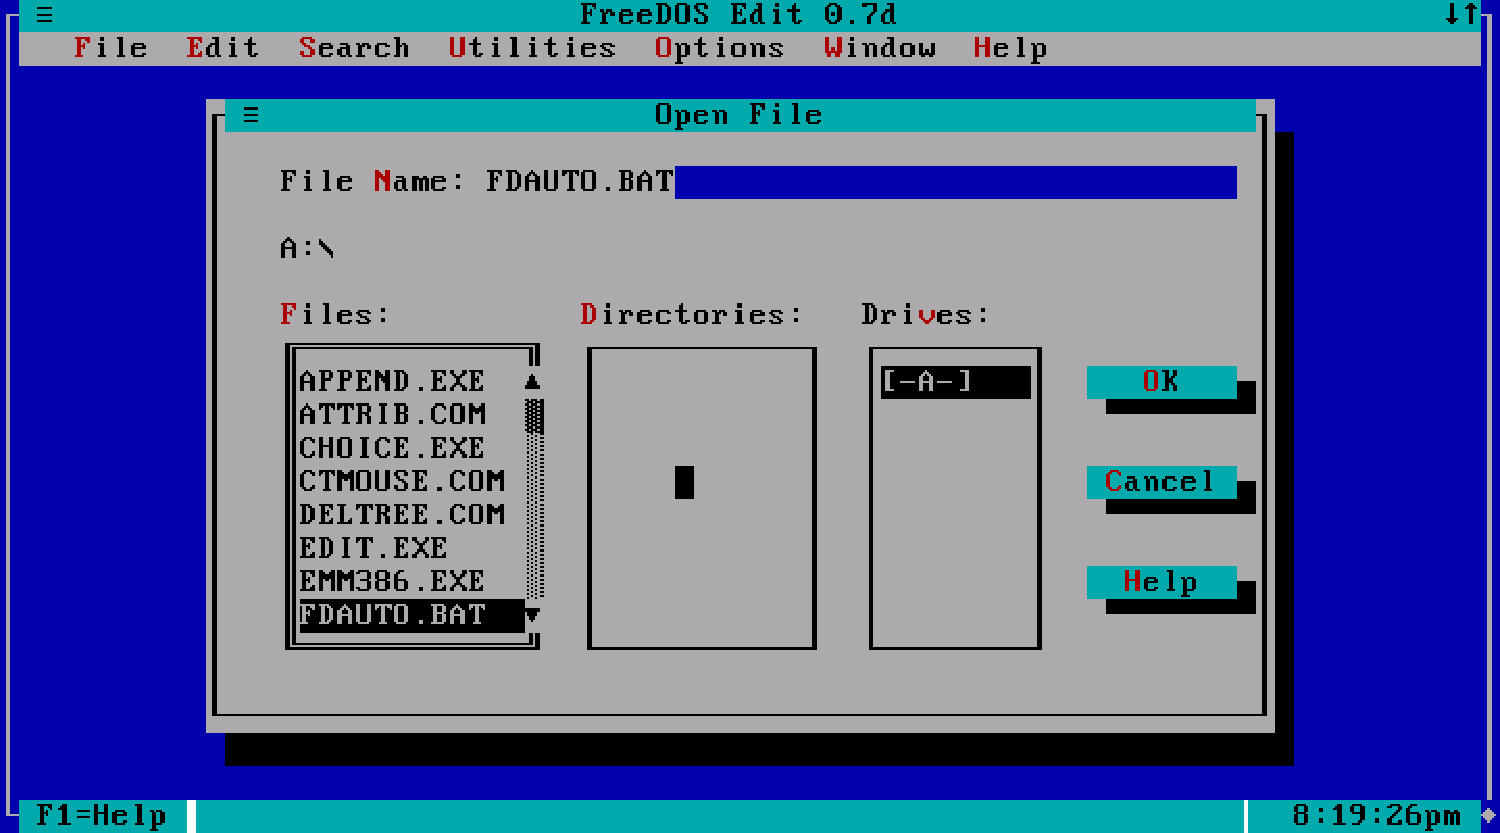
\includegraphics[width=1.0\textwidth]{./images/TUI}
	\caption{Textové uživatelské rozhraní -- FreeDOS Edit \cite{fdedit}}
	\label{fig:tui}
\end{figure}
% https://cs.wikipedia.org/wiki/Textov%C3%A9_u%C5%BEivatelsk%C3%A9_rozhran%C3%AD
% https://commons.wikimedia.org/wiki/File:Fdedit.png

Shellem se obecně myslí uživatelské prostředí pro využívání funkcí jádra operačního systému. V~této práci budeme slovem shell označovat právě interpret příkazů v~příkazové řádce. Je to program ovládaný příkazy, který umí spouštět ostatní programy a zajišťovat jejich vstup a zobrazovat jejich výstup.

%---

Prompt je krátký řetězec znaků, který se objeví na začátku řádky, do které se bude vepisovat příkaz v~příkazové řádce. Je používán k~zobrazování důležitých informací, jako například, ve kterém adresáři se uživatel nachází či jaké je jméno počítače, na kterém se nachází. Základní prompt v~operačním systému Ubuntu \cite{ubuntu} je v~ukázce \ref{lst:prompt}. Je zde ukázka jak vypsaného promptu, tak i jeho nastavení v~proměnné \texttt{PS1}.

\noindent
\begin{minipage}{\linewidth}
\begin{lstlisting}[language=bash, caption={Prompt v~shellu}, label={lst:prompt}]
n@t:~/Dropbox/g/nesrotom-dip-2016$ echo "$PS1"
\[\e]0;\u@\h: \w\a\]${debian_chroot:+($debian_chroot)}\[\033
[01;32m\]\u@\h\[\033[00m\]:\[\033[01;34m\]\w\[\033[00m\]\$
\end{lstlisting}
\end{minipage}

% http://www.linfo.org/prompt.html

%---

GNU \cite{gnu} je projekt zabývající se tvorbou a propagací svobodného software. Cílem je vytvořit kompletní svobodný operační systém unixového typu. Protože jádro operačního systému od GNU s~názvem Hurd \cite{hurd} nebylo tak úspěšné, začalo se používat jádro Linux \cite{linuxkernel}. Kombinace operačního systému GNU a jádra Linux se označuje jako GNU/Linux. GNU vytvořilo i svůj shell, Bash \cite{bash}. Sada základních příkazů, jejichž existence je předpokládána v~nějaké formě na každém operačním systému, se jmenuje GNU Coreutils \cite{coreutils}. Patří do ní příkazy jako \texttt{ls}, \texttt{cp}, \texttt{rm}, atd. Je důležité si uvědomit, že příkazy jako \texttt{cd}, \texttt{echo} jsou vestavěné příkazy shellu Bash, nikoliv samostané programy.

% https://www.gnu.org/software/bash/
% https://www.gnu.org/software/coreutils/coreutils.html

Terminál byl z~historického hlediska elektronické zařízení k~základní komunikaci s~počítačem. Dnes se v~operačních systémech spouští terminálové emulátory, ve kterých lze spustit různé programy. Nejčastěji je to právě shell.


Provádění příkazů můžeme rozdělit na dvě kategorie. Jednou z~nich je interaktivní režim, kdy interpret spouští příkazy tak, jak je uživatel píše do příkazové řádky. V~tomto režimu může uživatel také používat klávesové zkratky, aliasy, automatické doplňování a další funkce v~interaktivním režimu. Druhou kategorií je dávkový režim, kdy uživatel nejprve příkazy napíše do souboru. Takovému souboru obsahujícímu příkazy se říká skript. Takový soubor může být zavolán interpretem shellu, který postupně vykoná všechny příkazy. Tento postup se hodí pro složitější a opakující se příkazy.

%---

Debuggování je činnost, při které se v~kódu hledají chyby. Nejčastějším způsobem je zastavování programu na nějakém místě při vykonávání a následně zkoumání výstupů a nastavení proměnných za účelem najít něco, co je špatně. Také lze program nebo skript spouštět po jednotlivých příkazech, takovému postupu se říká krokování.

%---

\texttt{trap} je příkaz v~shellu, který spustí nějaký kód, pokud shell přijme signál, pro který byla \texttt{trap} nastavena. V~ukázce \ref{lst:trap} je spuštěn skript, který nastaví trap při ukončení programu signálem. V~Bashi je možné nastavit \texttt{trap} pro debuggování skriptů. Taková \texttt{trap} je spuštěna před každým příkazem.

\noindent
\begin{minipage}{\linewidth}
\begin{lstlisting}[language=bash, caption={Ukázka trap v~shellu Bash}, label={lst:trap}]
bash-4.3$ cat trap_example.sh
#!/bin/bash

clean() {
	echo "cleaning!"
}

trap clean SIGHUP SIGINT SIGTERM

sleep 5
bash-4.3$ ./trap_example.sh
^Ccleaning!
bash-4.3$ ./trap_example.sh
bash-4.3$
\end{lstlisting}
\end{minipage}

%
\chapter{Historie shellu a dnešní využití}

V~této kapitole stručně shrneme historii rodin nejpoužívanějších operačních systémů a shellů, které se v~nich používají.

% Napsat o tom, ze bash je dneska nejcastejsi, protoze linux je vlastne GNU/Linux a bash je GNU bash. Zsh je lepsi snad uplne ve vsem. Sh, resp Dash je rychlejsi.

%
\section{Windows}

Operační systém Windows \cite{windows} je obecně uživatelsky přívětivější pro laické uživatele, protože skoro vše je možné nastavit přes grafické rozhraní. Ovšem ne vždy je grafické prostředí dostupné a příkazová řádka je pak jediná možnost, jak ovládat počítač.

Pro automatizaci a jako nástroj, ve kterém lze snadno skriptovat, nabízí Windows nejen svůj shell PoweShell, ale i nemodifikovaný Bash pro operační systém Ubuntu, který funguje ve Windows subsystému pro Linux \cite{windowscmd}.

% https://en.wikipedia.org/wiki/Shell_(computing)#Microsoft_Windows
% -> https://en.wikipedia.org/wiki/Windows_shell

\section{UNIX}

Unix je rodina operačních systémů, které zvládnou spustit více úkonů najednou a do kterých se v~jeden okamžik může připojit více uživatelů. Historie těchto systémů sahá až na konec sedmdesátých let, kdy v~Bell laboratořích firmy AT\&T byl v~jazyce C vytvořen systém UNIX, jehož název byl zaregistrován jako ochranná známka. Časovou osu ukazuje obrázek \ref{fig:unixhistory}. Specifikace Single UNIX Specification \cite{sus} je souhrn standardů, které operační systém musí splňovat a dodržovat, aby se mohl označovat za UNIX.

Filosofie Unixu je sada doporučení a pravidel, která vznikla postupem času dle zkušeností tvůrců Unixu. Filosofie Unixu zdůrazňuje tvoření jednoduchého, přehledného a hlavně snadno rozšiřitelného a znovupoužitelného softwaru. Váží si programátorova času více, než času práce počítače. Nejznámější pravidlo je tvořit programy, které dělají jen jednu věc a dělají jí správně, rychle a bez chyb. Takové programy lze použít jako filtry a skládat je za sebe. To se často používá v~příkazové řádce, kdy se pomocí rour spojují výstupy programů se vstupy jiných programů. Zdánlivě složitý úkol tak lze udělat rychle a efektivně bez nutnosti programování v~nějakém externím jazyce.


\begin{figure}
	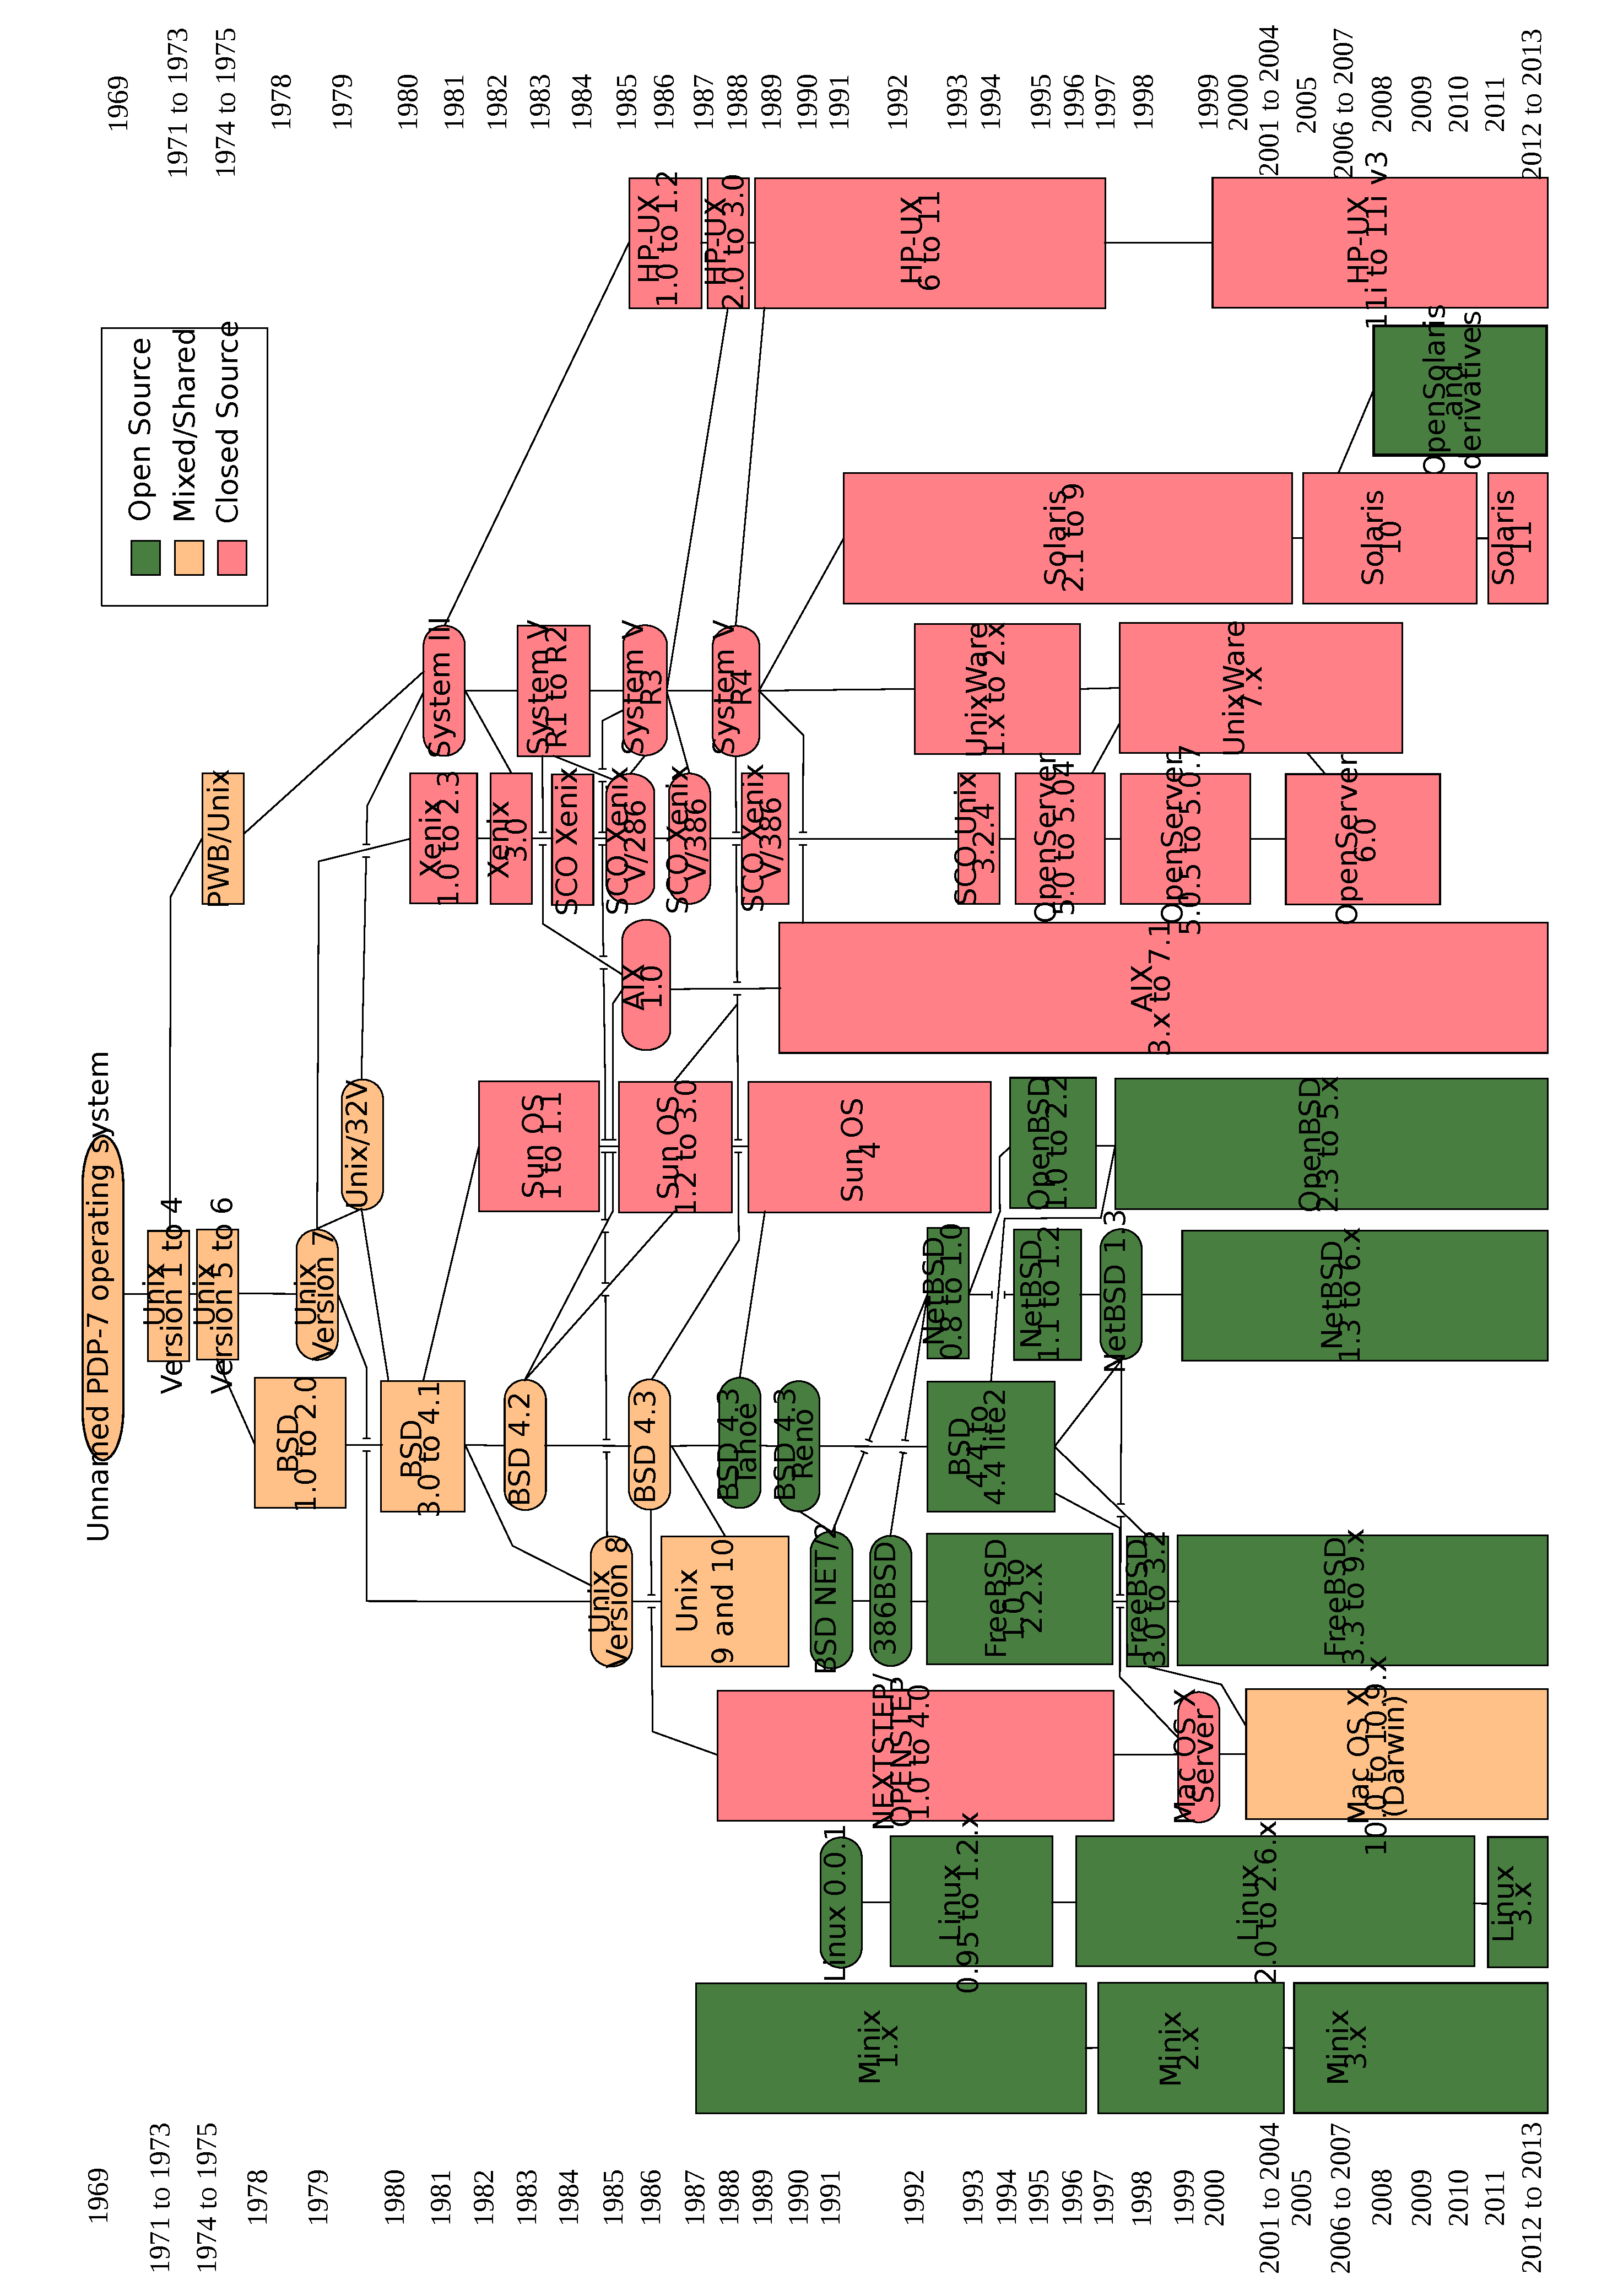
\includegraphics[width=1.0\textwidth]{./images/Unix_history-simple_rot_big}
	\caption{Historie unixu \cite{unixhistorysvg}}
	\label{fig:unixhistory}
\end{figure}

% https://en.wikipedia.org/wiki/File:Unix_history-simple.svg
% XXX: mozna https://simple.wikipedia.org/wiki/File:Unix_timeline.en.svg ?

% ZDROJ: https://edux.fit.cvut.cz/courses/BI-PS1/_media/lectures/01/bi-ps1-p01-introduction-01.pdf

\section{Linux}
Linux \cite{linux} je otevřený a svobodný Unix-like operační systém. Linuxem se obecně myslí GNU operační systém s~jádrem Linux. Unix-like znamená, že přestože je takový operační systém velice podobný systému Unix, nemá certifikaci \uv{Single UNIX Specification}. Linuxová distribuce je GNU/Linuxový systém, který většinou obsahuje balíčkovací systém, kterým je snadné doinstalovat ostatní programy. Linuxové distribuce jsou i předpřipravené, s~grafickým prostředím.


% https://www.amazon.com/Just-Fun-Story-Accidental-Revolutionary/dp/0066620732

% unix timeline for students
% http://unix.harley.com/instructors/timeline.html
% http://www.harley.com/books/sg3.html

% Recommended UNIX Books
% http://www.it.northwestern.edu/research/user-services/sscc/booklist.html

% https://www.goodreads.com/book/show/104745.The_Art_of_UNIX_Programming

\section{Shell}

Shell je uživatelské prostředí, ve kterém lze spouštět příkazy a využívat funkce jádra operačního systému. Shell se stará o~předávání vstupů a zobrazování výstupů takových programů, pokud této funkce využívají.

Obrázek \ref{fig:shell_history} ukazuje základní dělení Unixových shellů v~časové ose. Některé z~těchto shellů budou probrány v~dalších podkapitolách.

\begin{figure}[htb]\centering
	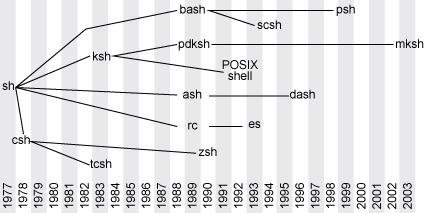
\includegraphics[width=\textwidth]{./images/tmp_shell_history}
	\caption{Historie Unixového Shellu \cite{historyofshells}}
	\label{fig:shell_history}
\end{figure}

O~shellu se říká slovní hříčka v~angličtině: If you hold a UNIX shell to your ear, can you hear the C? Shell označuje mořskou mušli a~C se vyslovuje jako moře. Je to analogie na to, že UNIX je napsaný v~jazyce C a~je shell je branou, skořápkou, do tohoto systému.

% V latexovych komentarich jsou nejake odkazy o historii.

% uvod, prehled csh, ksh, bash.
% https://www.ibm.com/developerworks/library/l-linux-shells/

% clanek od bourna z 1983, uvod do shellu, drtiva vetsina plati i dneska
%https://ia800300.us.archive.org/1/items/byte-magazine-1983-10/1983_10_BYTE_08-10_UNIX.pdf

% puvodni shell z unix v6
%https://github.com/JNeitzel/v6shell


\section{cmd.exe}

Shellem v~operačním systému MS-DOS a PC-DOS byl COMMAND.COM, 16-bitový intepretr příkazů. V~novějších systémech Windows byl tento shell nahrazen CMD.EXE \cite{windowsshell}, 32-bitovým interpretem příkazů. V~CMD.EXE byla dostupná emulace COMMAND.COM pro zpětnou kompatibilitu.

Tato příkazová řádka, shell, již umí přesměrovávat vstupy a výstupy, a~to jak do souboru, tak mezi procesy. Také je schopná vykonávat příkazy ze souborů, které se nazývají dávkové a zpravidla mívají příponu \texttt{bat}.

% https://en.wikipedia.org/wiki/COMMAND.COM

% https://en.wikipedia.org/wiki/PowerShell
% https://technet.microsoft.com/en-us/library/bb490954.aspx

\section{PowerShell}

Protože je základní příkazová řádka Windows omezená, co se funkcionality týče, existují další shelly pro operační systémy Windows, často i s~otevřeným zdrojovým kódem. Firma Microsoft chtěla vytvořit i svůj shell, který bude umět více věcí. S~jeho vývojem začala v~roce 2002 a po 3 letech jej zveřejnila jako Microsoft Command Shell (MSH) s~krycím jménem Monad, který byl později přejmenován na PowerShell.

PowerShell je integrován s~platformou .NET \cite{windowsdotnet} od Microsoftu. Je tedy možné využívat již vytvořené funkce a nástroje, které usnadní a urychlí vývoj.

Oproti cmd.exe umí PowerShell mnoho věcí. PowerShell umožňuje spouštět příkazy v~intervalech nebo v~nějaký přesný čas. Přibyly konstrukce pro větvení. Příkazy je možné spouštět na pozadí nebo vzdáleně.


% https://technet.microsoft.com/en-us/library/2005.11.scripting.aspx
% http://www.makeuseof.com/tag/command-prompt-vs-windows-powershell-whats-difference/


\section{V9 -- Thomson Shell}

První shell pro systém UNIX napsal Ken Thomson v~roce 1971 a byl nazván V9 shell. Jednalo se již o~uživatelský program, tedy spuštěný mimo jádro operačního systému. Shell byl velice jednoduchý a některá základní funkcionalita byla umožněna až dalšími programy. Například expanze parametrů byla zajišťována příkazem glob. Základní větvení, if, bylo také jako samostatný program.

V9 shell přinesl syntaxi pro přesměrování a pipelining. Uměl spouštět více oddělených příkazů a dokázal příkazy spouštět na pozadí. Naopak třeba chyběla podpora pro spouštění skriptů.

Díky jednoduchosti a oddělenosti ostatní funkcionality měly zdrojové kódy pouze 900 řádek v~jazyce C.

Originální zdrojové kódy jsou stále dostupné \cite{thompsonshell}. Projekt Osh \cite{v6shell}, obsahuje jak port tohoto původního shellu, tak i jeho vylepšenou verzi.


% TODO: cite book https://en.wikipedia.org/wiki/The_Unix_Programming_Environment
% http://cs.uwec.edu/~buipj/teaching/cs.388.s14/static/pdf/upe.pdf

%
%
%
\section{Sh -- Bourne Shell}

Bourne shell byl vytvořen pro UNIX V7 v~roce 1977 Stephenem Bournem v~laboratořích Bell a AT\&T. Na rozdíl od Thomsonova v9 shellu umí Bourne shell spouštět příkazy ze souborů, skriptů. Šlo tedy psát znovupoužitelné sady příkazů, které zjednodušily a urychlily vývoj různých aplikací. Interaktivní režim je samozřejmě podporován také.

Bourne shell přinesl také podporu smyček, proměnných, signály, subshelly a HERE dokumenty. Skripty v~shellu mohly sloužit i jako filtry. Z~tohoto shellu poté začaly vznikat další, jak je vidět na obrázku \ref{fig:shell_history}.

Dnes se Bourne shell a jeho jiné implementace stále používají. Je totiž menší, rychlejší a stabilnější než ostatní shelly. Má také minimum závislostí na externích knihovnách.

%
%
%
\section{Dash -- Debian Almquist Shell}

Dash je moderní implementace Bourne Shellu. Snaží se být stále malý a rychlý, ale přesto bezpečný a stabilní při chybách systému. Důležitý je fakt, že tento shell splňuje standardy POSIX 1003.2 a 1003.2a, tedy standardy o~regulárních výrazech, respektive jak se má chovat shell a~jeho základní nástroje.

Tento shell byl nastaven jako shell, který spouští příkazy při bootování i~skripty, které mají jako shebang \texttt{/bin/sh} na operačních systémech Ubuntu a~Debian.

Shebang je cesta k~programu, který má interpretovat skript. Tato cesta se píše na první řádek skriptu a je uvozena znaky \texttt{\#!}.

% $\#!$.

% todo: citovat:?
% https://standards.ieee.org/findstds/standard/1003.2a-1992.html
% \url{https://www.in-ulm.de/~mascheck/various/ash/#dash}
% \url{https://cs.wikipedia.org/wiki/Debian_Almquist_shell}
% \url{https://wiki.archlinux.org/index.php/Dash}
% https://wiki.ubuntu.com/DashAsBinSh


%
%
%
\section{Csh -- C Shell}

C Shell byl vytvořen Billem Joyem v~sedmdesátých letech. Hlavní myšlenkou byla syntaxe více podobná jazyku C. Dnes se používá vylepšená verze tcsh \cite{tcsh}.

Přestože v~v~dnešní době tento shell není moc oblíbený, při svém vzniku představil některé nové vlastnosti, které pak začaly adaptovat i~ostatní shelly. Byla to například historie příkazů nebo podpora aliasů.

% http://www.tcsh.org/
% https://en.wikipedia.org/wiki/C_shell



%
%
%
\section{Ksh -- Korn Shell}

Korn Shell \cite{ksh} je Unixový shell, který vytvořil David Korn a jeho kolegové z~Bell laboratoří na začátku osmdesátých let. Korn Shell byl vyvíjen z~Bourne Shellu a~zachovává zpětnou kompatibilitu.

Korn Shell umožnuje upravovat psaný příkaz jako v~editorech Vi nebo Emacs. Podporuje spravování spuštěných programů, historie a~aliasy příkazů byly převzaty z~C Shellu. Korn Shell dovoluje vytvářet asociativní pole a~umí pracovat s~desetinnými čísly.

% https://en.wikipedia.org/wiki/KornShell

%
%
%
\section{Bash -- Bourne Again Shell}

Bash \cite{bash} \cite{learningthebashshell} \cite{unixprogrammingenvironment} je open source shell projektu GNU. Bash se snaží být zpětně kompatibilní s~Bourne shellem, tedy skripty napsané v~Bourne shellu pravděpodobně půjdou spustit i v~Bashi. Naopak to je problém, který se řeší programem \texttt{checkbashisms}, o~kterém bude řeč dále.

Bash obsahuje konstrukty pro smyčky. Nejen smyčky \texttt{while} a \texttt{for}, ale i \texttt{until}, což je obdoba smyčky \texttt{do-while} v~jazyce C. Pro větvení lze použít klasický příkaz \texttt{if}, ale například i \texttt{case}, což je obdoba \texttt{switch} v~jazyce C.

Z~C Shellu Bash převzal například expanzi znaku tilda, kdy se \textasciitilde{} změní na obsah proměnné \$HOME. Další funkce z~C Shellu je například zásobník adresářů, nebo práce s~historií.

Z~Korn shellu bash převzal například příkaz \texttt{fc}, pro volání a opravování příkazů z~historie. Pak je to třeba příkaz \texttt{type}, který vypíše typ příkazu. V~ukázce \ref{lst:bashtype} je vidět rozdíl mezi vnitřním příkazem Bashe.

\noindent
\begin{minipage}{\linewidth}
\begin{lstlisting}[language=bash, caption={Příkaz type v~Bashi}, label={lst:bashtype}]
n@t:~$ type echo
echo is a shell builtin
n@t:~$ type rm
rm is aliased to `csfunc_rm'
n@t:~$ type grep
grep is aliased to `grep --color=auto'
\end{lstlisting}
\end{minipage}

Protože je Bash shellem z~projektu GNU, je často základním uživatelským přihlašovacím shellem. Bash je právě proto většinou prvním shellem, se kterým se nový uživatel potká.

% https://www.cs.indiana.edu/docproject/shells/bash/features.html

% !!!
% http://www.aosabook.org/en/bash.html?cm_mc_uid=36339891185014923692137&cm_mc_sid_50200000=1492436376


%
%
%
\section{Zsh -- Z~Shell}

Z~Shell \cite{zsh} je Unixový shell pojmenovaný po přihlašovacím jménu profesora z~Yale, Zhong Shao. Byl napsán v~roce 1990 Paulem Falstadem.

Z~Shell nejenom že nabízí nejvíce funkcí mezi používanými Shelly pro Unixové systémy, ale také je kolem něj velká aktivní komunita spravující mnoho pluginů, v~čele s~Oh My Zsh \cite{ohmyzsh}, o~kterém bude řeč dále.

Funkcí navíc oproti ostatním shellům je hodně. Hned po instalaci Z~Shellu se uživateli nabídne možnost nastavení, jako například nastavení ukládání historie, nebo automatické doplňování. Z~Shell má na rozdíl od Bashe nativní podporu automatického doplňování, která je nejen rychlejší, obsahuje více způsobů, jak s~ní iteragovat, ale je i snadnější na implementaci do uživatelských skriptů.

Z~Shell umožňuje zobrazit hodnotu promptu \texttt{PS1} i vpravo. Tím se otevírají další možnosti pro zobrazování informací v~okně terminálu. Toto místo často bývá nevyužité, protože příkazy nejsou většinou tak dlouhé.

Ukládání historie je automaticky sdíleno mezi jednotlivými instancemi Z~Shellu. Takové chování je možné nastavit i například v~Bashi, ale je pro to potřeba ukládat každý příkaz do souboru na disk.

Další z~věcí ovlivňujících pohodlnost práce v~Z~Shellu je takzvaný globbing, který je lepší než v~ostatních shellech. Jedná se o~popsání jednoho, nebo několika řetězců, zpravidla názvu souborů, kratším zápisem. Například \texttt{*.txt} se zamění za všechny soubory ve složce s~příponou txt. V~Z~Shellu je ale možné popsat cestu k~souboru pomocí zkratek a nechat ji doplnit. Například \texttt{/h/u/t/s} se změní na \texttt{/home/user/test/script.sh}.

Velmi užitečnou funkcí je automatická oprava překlepů. V~Bashi je velmi limitovaná oprava příkazů, ale v~Z~Shellu se opravují nejen názvy příkazů, ale také argumentů. Pokud je argumentem cesta k~souboru, který neexistuje, Z~Shell navrhne cestu k~souboru, který existuje a má podobnou cestu.

Přestože Z~Shell se zdá být ve všech směrech lepší než Bash, tak není základním shellem ve většině Linuxových distribucích.

% \url{http://zsh.sourceforge.net/FAQ/}

%
%
%
\section{Práce v~příkazové řádce}

Práce v~příkazové řádce může být mnohem efektivnější na rozdíl od práce v~grafickém prostředí. Při normální práci není tolik nutné používat myš. Složitější, nebo méně používané funkce a programy je zpravidla rychlejší napsat, než vyhledat v~nějakém kontextovém menu. To samozřejmě platí až tehdy, kdy uživatel ví, jakým příkazem a s~jakými parametry se příkazy spouští.

Nový uživatel, který ještě není s~prací v~příkazové řádce zběhlý, bude ze začátku méně efektivní, ale časem si základní příkazy zapamatuje a jeho efektivita bude růst.

Další výhodou je možnost používání příkazů ve formě filtrů. I~složitou věc je často možné vyřešit pomocí spuštění několika příkazů v~rouře za sebou. Příkazy v~mezikrocích mohou být také uživatelské skripty.

Velice snadná je také automatizace. Pokud uživatel často potřebuje vykonat nějakou sekvenci příkazů, může složené příkazy vyhledat v~historii a například z~nich vytvořit skript.

Nevýhodou na rozdíl od práce v~grafickém prostředí je často fakt, že zpravidla ne všechny potřebné informace jsou stále na očích. Tento problém lze vyřešit rozšířeným a vylepšeným promptem, nebo takovými emulátory terminálů, které mohou vyhradit nějakou část terminálu pro zobrazování informací. I~přesto se stává, že uživatel musí často spouštět nějaké příkazy, které vypíšou nějaké informace, aby věděl stav věcí, které ho zajímají.

S~rychlejší prací přichází také větší zodpovědnost za spuštěné příkazy. Překlep v~příkaze, který provádí nějaké změny, může způsobit komplikace. Některé programy se uživatele dotazují, zdali chce operaci opravdu provést, ale není to pravidlem. Nejlepší prevencí je si tedy příkaz před spuštěním překontrolovat.


%
%
%
\section{Nastavení shellu}

GNU/Linuxové distribuce, které nabízejí předpřipravené prostředí, mají pro výchozí shell bash připravené takzvané rc soubory, které nějakým způsobem upravují běžící interaktivní shell. Jednou z~nejviditelnějších změn je nastavení proměnné \texttt{PS1}, o~které bude řeč v~pozdější kapitole, která určuje styl promptu. Ve výchozím nastavení Bashe, tedy po spuštění Bashe bez načtení rc souborů, které lze spustit pomocí příkazu bash \texttt{--norc}, se v~\texttt{PS1} zobrazuje pouze název shellu, jeho verze a zdali je uživatel root. Po načtení výchozích rc souborů se v~\texttt{PS1} ukazují informace, jako jsou jméno uživatele, jméno počítače a~co je velmi důležité, jméno aktuálního adresáře.

Tyto informace jdou snadno získat použitím některých základních příkazů, například whoami, hostname, pwd. Protože tyto informace jsou důležité a~potřebujeme je vědět pořád, chceme je mít pořád na očích.

Mezi další základní nastavení shellu patří i aliasy. Jedná se o~zkratky, které se před vykonáním nahradí za řetězec, který nahrazují. V~ukázce \ref{lst:alias} je příklad aliasů pro příkaz \texttt{ls}. Příkaz \texttt{ls} patří k~velmi základním a jeho účelem je vypsat obsah složky. V~základním nastavení, bez argumentů předaných při volání, se vypíšou pouze názvy souborů. To může být vhodné v~nějakých skriptech, ale uživatel v~příkazové řádce chce takovou informaci zobrazit přehledně a~barevně.

\noindent
\begin{minipage}{\linewidth}
\begin{lstlisting}[language=bash, caption={Příklad použití aliasu v~Bashi}, label={lst:alias}]
n@t:~$ type l
l is aliased to `ls -CF'
n@t:~$ type ll
ll is aliased to `ls -alF'

n@t:/tmp/ls$ ll
total 28
drwxrwxr-x  3 n    n     4096 kve  2 15:20 ./
drwxrwxrwt 12 root root 20480 kve  2 15:19 ../
-rw-rw-r--  1 n    n        0 kve  2 15:19 a.txt
-rw-rw-r--  1 n    n        0 kve  2 15:19 b.txt
-rw-rw-r--  1 n    n        0 kve  2 15:19 c.txt
drwxrwxr-x  2 n    n     4096 kve  2 15:20 d/
\end{lstlisting}
\end{minipage}

%
%
%
\section{Terminál}

% Terminál byl z historického hlediska elektronické zařízení k základní komunikaci s počítačem. Dnes se v operačních systémech spouští terminálové emulátory, ve kterých lze spustit různé programy. Nejčastěji je to právě shell.

Protože je terminál elektronické zařízení, ukážeme zde pouze emulátory takových terminálů.

Prvním druhem jsou programy, které vytvoří nové okno v~desktopovém prostředí operačního systému. Na operačních systémech Linux je to zpravidla X Window System \cite{xorg}.

Druhým druhem jsou programy, které se spustí už v~nějakém terminálu a emulují další terminál. To se hodí například při vzdálené práci. Takový emulátor běží na straně serveru a pokud se přeruší spojení, terminál zůstane neporušen.

Obrázek \ref{fig:terminal_invert} ukazuje okno GNOME Terminal v~grafickém prostředí LXDE s~instancí terminálového emulátoru GNU Screen.

\begin{figure}[htb]\centering
	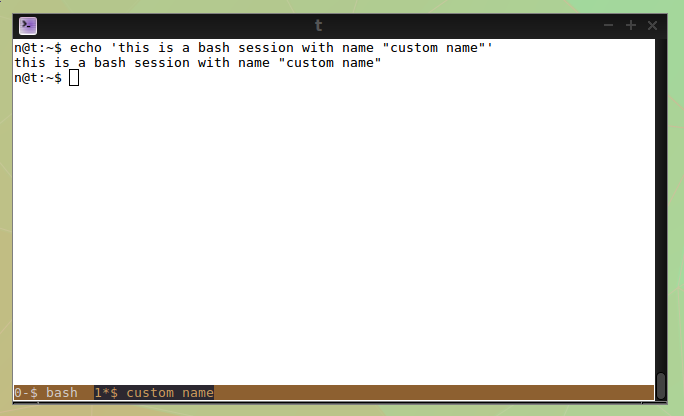
\includegraphics[width=\textwidth]{./images/terminal_invert}
	\caption{LXTerminal s~emulátorem terminálu GNU Screen}
	\label{fig:terminal_invert}
\end{figure}

% https://en.wikipedia.org/wiki/List_of_terminal_emulators

%-----------------------------------------------------------------------------


% Napsat o tom, ze cilem prace je usnadnit praci v prikazove radce a sepsat zakladni funkcionalitu debuggeru.


\section{Existující řešení}

Awesome \cite{awesome} je název Git repozitáře se seznamem různých zajímavých řešení ze světa svobodného software. Je zde i podsekce awesome-shell \cite{awesomeshell}, ve které lze nalézt spoustu užitečných nástrojů pro práci s~příkazovou řádkou, nebo psaním skriptů v~Bashi.

Spousta těchto nástrojů je nad rámec této práce. Představíme si zde některé základní nástroje pro vylepšení interaktivního shellu, nebo nástrojů a~frameworků pro psaní shell skriptů.

% github.com/sindresorhus/awesome
% github.com/alebcay/awesome-shell

\section{Bash frameworky pro psaní skriptů}

Existuje mnoho projektů, jejichž cílem je vytvořit framework v~bashi, který má nějakým způsobem zjednodušit vytváření především větších skriptů v~bashi. Spousta dnešních vývojářů je zvyklá na objektově orientovaný přístup k~programování a je tedy pro těžké vytvořit větší program, který by zůstal přehledný.

\subsection{Bash Infinity Framework}
Bash Infinity Framework \cite{bashinfinity}, známý také jako Bash OO framework \cite{bashooframework}, je framework napsaný v~Bashi, který umožňuje vytvářet třídy, výjimky a testy. Cílem je nabídnout možnost skriptovat v~Bashi objektově. Takový kód potom může být přehlednější a modulárnější.

% \url{github.com/niieani/bash-oo-framework}
% https://invent.life/project/bash-infinity-framework
%
%
%
%
%

\section{Bash frameworky pro správu doplňků}

Existuje spousta věcí, které uživatel příkazové řádky potřebuje občas řešit. Řešení pro daný problém je víc. Buď si uživatel vyřeší problém sám, nebo bude hledat řešení na internetu. Nástroje do shellu, které umí i spravovat doplňky, mohou mít řešení pro daný problém. Instalace a použití pak bude velmi jednoduché, intuitivní a bude zde nějaká záruka o~funkčnosti a kvalitě.

Přestože je tato práce převážně o~shellu Bash, pro Z~Shell existuje nástroj Oh My Zsh, který je jeden z~nejpokročilejších a s~největší uživatelskou základnou.

%
%
%
\subsection{Oh My Zsh}

Oh My Zsh \cite{ohmyzsh} je nástroj pro Z~shell. Má otevřený kód a je vyvíjen komunitou. Jeho cílem je spravovat konfiguraci Z~Shellu. Lze přes něj instalovat spoustu doplňků, ať se jedná o~barevné schéma v~terminálu, nebo nástroje pro lepší práci s~verzovacími systémy.

Ukázkou takového barevného schématu je obrázek \ref{fig:zsh_theme}.

\begin{figure}[htb]\centering
	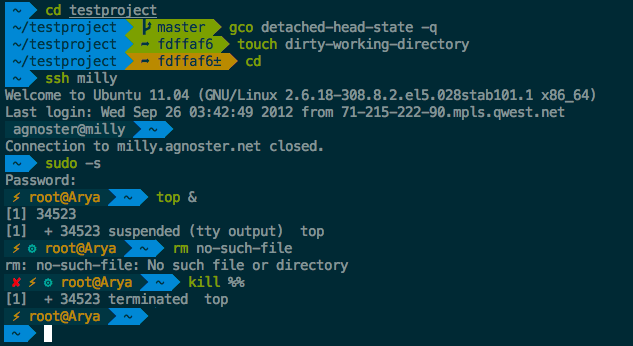
\includegraphics[width=\textwidth]{./images/zsh_theme}
	\caption{Barevné schéma do Z~Shellu \cite{ohmyzshimg}}
	\label{fig:zsh_theme}
\end{figure}

% http://ohmyz.sh

% TODO vic ukazek?

%
%
%
\subsection{Bash-it}

Bash-it \cite{bashit} je nástroj pro Bash, který nabízí podobné funkce jako Oh My Zsh. Nabízí instalaci barevných schémat a doplňků pro práci v~různých programech.

Bash-it není tak populární hlavně proto, že Z~Shell umí více funkcí. Pokud chce mít uživatel velmi pokročilý a nastavený shell, sáhne raději po Z~Shellu a Oh My Zsh.


% http://itsfoss.com/bash-it-terminal-tool/
% \url{http://github.com/Bash-it/bash-it}
%

%
%
%
\section{Bash frameworky pro úpravu promptu}

\subsection{Liquid Prompt}

Projekt Liquid Prompt \cite{liquidprompt} nastaví adaptivní prompt v~interaktivním Bashi. Myslí se tím, že se v~promptu zobrazí informace až tehdy, je-li relevantní.

Příkladem může být práce s~verzovacím systémem, kdy se uživatel například přepíná mezi větvemi software. Nebo to může být náhlé zatížení procesoru.

% github.com/nojhan/liquidprompt

\subsection{Sexy Bash Prompt}

Projekt Sexy Bash Prompt \cite{sexybashprompt} je další používaný prompt v~interaktivním Bashi. Umožňuje vypisovat informace o~stavu větví ve verzovacím systému Git. Obrázek \ref{fig:sexy_prompt} ukazuje příklad takového promptu.

\begin{figure}[htb]\centering
	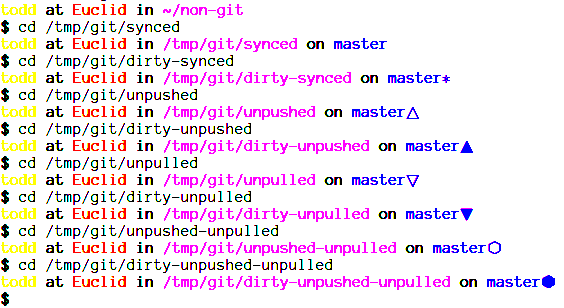
\includegraphics[width=\textwidth]{./images/sexy_prompt_edited}
	\caption{Ukázka Sexy Bash Prompt \cite{sexybashprompt}}
	\label{fig:sexy_prompt}
\end{figure}

% https://github.com/twolfson/sexy-bash-prompt

%------------------------------------------------------------------------------


%
%
%
\chapter{Analýza a návrh}

%
%
%
\section{Cíl práce}

Prvotním cílem práce bylo navrhnout a vytvořit shell, který bude asistovat studentům na začátku jejich studia shellu. Takový shell by je měl upozorňovat na chyby a navrhovat lepší řešení. Přitom mělo být maximálně využito existujících řešení.

Protože nástroj na upozorňování chyb, konkrétně vynikající ShellCheck, již existuje, byla část cíle práce nastavena obecněji na analýzu a ovlivňování příkazů spouštěných z~interaktivní příkazové řádky. Tím se v~praxi myslí vytvořit nástroj, který dokáže spustit skripty před vykonáním příkazu a být je schopen ovlivnit, nebo zabránit jejich vykonávání.

Spouštění příkazů, které byly nesprávně použity, může vést k~provedení nechtěné akce. Proto je dalším cílem práce je vytvořit sadu upravených základních programů z~GNU Coreutils, které uživatele nejprve upozorní na změny, které nastanou po spuštění takového příkazu a možnost vrátit stav změněných věcí do původního stavu.

Posledním cílem je vytvořit jednoduchý debugger příkazů spouštěných v~interaktivním shellu. Na rozdíl od normálních debuggerů pro shell skripty, například bashdb -- BASH Debugger, je cílem takového debuggeru maximální jednoduchost použití. Tím se například myslí spuštění debuggeru s~předepsaným posledním příkazem pomocí spuštění jediného příkazu.

Nejdůležitějším cílem práce je vytvořit takový nástroj, který bude neinvazivní při normálním používání příkazové řádky. Nástroj, který bude začátečník intenzivně využívat, zatímco pokročilý uživatel ho bude mít na pozadí a čas od času ho upozorní na nějakou chybu, popřípadě mu pomůže urychlit práci na nějakém nesprávně fungujícím příkazu.

%
%
%
\section{Fungování shellu}

Abychom mohli implementovat jak hooky před a po příkazech, tak přepsat chování základních příkazů z~GNU Coretutils, je potřeba znát základní procesy, které se dějí při vykonávání příkazů.

Tyto postupy platí pro shell Bash, ale jsou velice podobné i v~ostatních Unixových shellech.

%
%
%
\subsection{Životní cyklus příkazu}

V~této kapitole vysvětlíme, co všechno všechno důležitého se stane mezi tím, kdy shell přijme příkaz a než je skutečně vykonán.

\begin{figure}[htb]\centering
	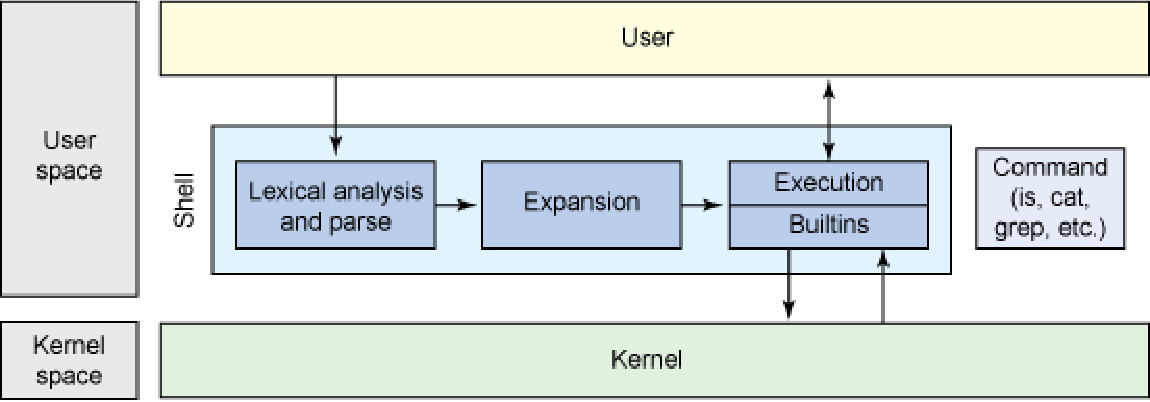
\includegraphics[width=\textwidth]{./images/shell_arch2}
	\caption{Architektura shellu \cite{historyofshells}}
	\label{fig:shell_arch}
\end{figure}


Prvním krokem je escapovaní, neboli převod znaků, které mají ve svém kontextu speciální význam. V~shellu lze tento postup provést pomocí znaku \texttt{\textbackslash}, nebo tím, že řetězec znaků dáme do uvozovek. Příkladem může být znak \texttt{\#}, který značí, že znaky za ním jsou pouze komentář. V~ukázce \ref{lst:escape} jsou čtyři příklady zavolání příkazu echo. V~prvním případě ale znak \# není vyescapován a Bash ho vyhodnotí jako začátek komentáře, proto se vypíše jen část, oproti ostatním voláním.

% TODO: pridat strong/weak quoting?
% http://wiki.bash-hackers.org/syntax/quoting
\noindent
\begin{minipage}{\linewidth}
\begin{lstlisting}[language=bash, caption={Escapovaní v~shellu}, label={lst:escape}]
$ echo a # b
a
$ echo a \# b
a # b
$ echo "a # b"
a # b
$ echo 'a # b'
a # b
\end{lstlisting}
\end{minipage}

Druhým krokem je odstranění komentářů. V~Bashi lze nastavit, aby se v~interaktivním shellu komentáře ignorovaly. Slouží k~tomu proměnná \texttt{interactive\_comments}, v~základním nastavení jsou komentáře zapnuté.

Třetím krokem je rozdělení celého vstupu na příkazy. K~příkazům patří přesměrovávání vstupů a výstupů. Jednoduchý příkaz je označení buď pro přiřazení proměnné, nebo název příkazu. Příkazů v~jednom vstupu může být více. Příkazy mohou být za sebou v~rouře, odděleny logickým and nebo or. Příkazy mohou být také odděleny jednoduše pomocí středníku, nebo v~případě spouštění ze skriptu i novou řádkou. Stejně může příkazy rozdělovat ampersand, který značí,  že se příkaz spustí na pozadí. Některé konstrukty již z~principu obsahují více příkazů, například podmínky nebo smyčky.

Čtvrtým krokem je expanze a substituce. Například znak tilda se nahradí za obsah proměnné \texttt{HOME}, proměnné se nastaví na své hodnoty. Pokud je součástí volání subshellu, zavolá se zde.

Posledním  krokem je samotné spuštění příkazu, popřípadě přiřazení do proměnné. O~spouštění příkazů pojednává kapitola \ref{sec:exec}.

Celý cyklus je také popsán v~diagramu \ref{fig:bash_diag}.

\begin{figure}[htb]\centering
	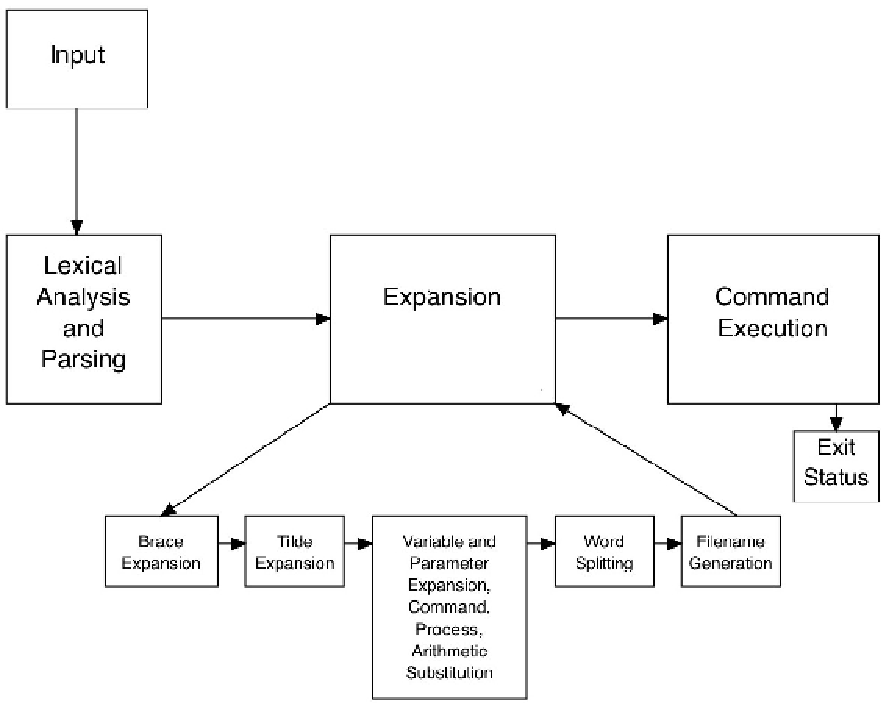
\includegraphics[width=\textwidth]{./images/bash-article-diagram}
	\caption{Bash diagram \cite{bashdiagimg}}
	\label{fig:bash_diag}
\end{figure}

% http://wiki.bash-hackers.org/syntax/expansion/intro


% https://edux.fit.cvut.cz/courses/BI-PS1/_media/lectures/02/bi-ps1-p02-cli-04.pdf

%
%
%
\subsection{Gramatika shellu}

Gramatika shellu je oproti ostatním jazykům jednoduchá, ale často nejasná. V~mnoha případech záleží na kontextu. Dokonce je možné vytvořit proměnnou s~názvem shodujícím se s~klíčovým slovem.

Popíšeme si zde pouze základ gramatiky. Pro více informací a detailní popis je dobré přečíst si manuálové stránky Bashe. Úplně kompletní gramatiku lze nalézt ve zdrojových kódech Bashe, konkrétně v~souboru \texttt{parse.y}.

Základem je jednoduchý příkaz, který začíná svým názvem a jeho další argumenty a přesměrování vstupů a výstupů jsou odděleny mezerou. Jednoduchý příkaz je ukončen kontrolním operátorem, které jsou v~ukázce \ref{lst:bashcontrol}.

\noindent
\begin{minipage}{\linewidth}
\begin{lstlisting}[language=bash, caption={Kontrolní operátory v~Bashi}, label={lst:bashcontrol}]
|| & && ; ;; ( ) | |& <newline>
\end{lstlisting}
\end{minipage}

Roura, anglicky pipeline, je sekvence jednoho, nebo více příkazů oddělených kontrolními operátory roury. Formát takového zápisu je v~ukázce \ref{lst:bashpipe}.

\noindent
\begin{minipage}{\linewidth}
\begin{lstlisting}[language=bash, caption={Formát roury v~Bashi}, label={lst:bashpipe}]
[time [-p]] [ ! ] command [ [|||&] command2 ... ]
\end{lstlisting}
\end{minipage}

Seznam příkazů, anglicky list, je sekvence příkazů nebo rour oddělených kontrolními operátory. Listy končící kontrolním operátorem ampersand jsou spuštěny na pozadí. Listy mohou být spojeny kontrolními operátory \texttt{and} nebo \texttt{or}. Podle návratových kódů se řídí vykonávání dalších příkazů v~listu.

Složené příkazy se dělí do více podkategorií. Zaprvé to jsou subshelly, které se označují jednoduchými závorkami. Dále to jsou podmíněné příkazy a~aritmetické bloky. Další kategorií jsou konstrukty měnící vykonávání příkazů a~smyčky, takže například \texttt{if} a~\texttt{while}. Formát smyčky \texttt{for} je v~ukázce \ref{lst:bashfor}.

\noindent
\begin{minipage}{\linewidth}
\begin{lstlisting}[language=bash, caption={Formát jedné varianty cyklu for v~Bashi}, label={lst:bashfor}]
for name [ [ in [ word ... ] ] ; ] do list ; done
\end{lstlisting}
\end{minipage}

% Soubor s gramatikiou bashe, parse.y, ma pres 6000 radek. Chtel bych zde napsat zjednodusenou gramatiku, ktera by se dala snadno pochopit (ono to zas tak slozite neni).
% v man bash je gramatika
% Popsat jakym zpusobem parsuje gramatiku BASH (yacc) a jakym to delaji parsery bashlex a bashast.



\subsubsection{Projekty parsující shell skripty}

%
\subsubsection{Beautysh}

Projekt Beautysh \cite{beautysh} si dává za cíl formátovat shell skripty tak, aby byly čitelnější. Jedná se o~malý a~jednoduchý projekt. Neprobíhá zde žádné parsování do abstraktního syntaktického stromu. Vstup je jen po řádcích rozlišován pomocí regulárních výrazů.

% Protože gramatika shellu může být bez kontextu nejasná, Beautysh si neporadí například s kódem \ref{lst:beautysh}

% \begin{lstlisting}[language=bash, caption={Beautifysh}, label={lst:beautysh}]
% done=3;echo done;done
% \end{lstlisting}

% \url{https://github.com/bemeurer/beautysh/blob/master/beautysh/beautysh.py}



%
%
%
\subsubsection{Bashlex}\label{sec:bashlex}

Bashlex \cite{bashlex} je knihovna napsaná ve skriptovacím jazyce Python \cite{Python}, která zjednodušeně imituje práci vnitřního parseru Bashe. Z~velké části se jedná jen o~přepsání zdrojových kódů Bashe z~jazyka C.

Existují zde rozdíly oproti parseru v~Bashi. Za prvé se nespouští žádné příkazy, knihovna umí pouze parsovat. Na rozdíl od parseru Yacc \cite{yacc}, který používá Bash, je Bashlex reentrantní. Výstupem Bashlexu je kompletní abstraktní syntaktický strom.

\noindent
\begin{minipage}{\linewidth}
\begin{lstlisting}[language=bash, caption={Výstup z~knihovny Bashlex}, label={lst:bashlex}]
$ python
>>> import bashlex
>>> parts = bashlex.parse('true && cat <(echo $(echo foo))')
>>> for ast in parts:
...     print ast.dump()
ListNode(pos=(0, 31), parts=[
  CommandNode(pos=(0, 4), parts=[
    WordNode(pos=(0, 4), word='true'),
  ]),
  OperatorNode(op='&&', pos=(5, 7)),
  CommandNode(pos=(8, 31), parts=[
    WordNode(pos=(8, 11), word='cat'),
    WordNode(pos=(12, 31), word='<(echo $(echo foo))', parts=[
      ProcesssubstitutionNode(command=
        CommandNode(pos=(14, 30), parts=[
          WordNode(pos=(14, 18), word='echo'),
          WordNode(pos=(19, 30), word='$(echo foo)', parts=[
            CommandsubstitutionNode(command=
              CommandNode(pos=(21, 29), parts=[
                WordNode(pos=(21, 25), word='echo'),
                WordNode(pos=(26, 29), word='foo'),
              ]), pos=(19, 30)),
          ]),
        ]), pos=(12, 31)),
    ]),
  ]),
])
\end{lstlisting}
\end{minipage}

% \url{https://github.com/idank/bashlex/blob/master/bashlex/parser.py}

%
%
%
\subsubsection{Libbash}

Libbash \cite{libbash} je projekt, který vzniknul v~roce 2010 na akci Google Summer of Code. Cílem je jako stejně u~knihovny Bashlex vytvořit ze vstupu kompletní abstraktní syntaktický strom.

Libbash je napsaný v~jazyce C++, ale využívá generátor parserů ANTLR \cite{antlr}, který je v~Javě. Gramatika Bashe je pro tento generátor popsána v~souboru \texttt{bashast.g}.

Projekt se stal i součástí Google Summer of Code v~roce 2011. Na stránkách operačního systému Gentoo \cite{gentoolibbash} je Libbashi věnovaná stránka, ale na Gitových repozitářích není již žádná nedávná aktivita. Protože má Libbash velký potenciál, je možné, že se projekt obnoví.


% https://qiaomuf.wordpress.com/2011/05/05/introduction-to-libbash/
% http://www.antlr.org/
% https://wiki.gentoo.org/wiki/Project:Libbash
% \url{https://github.com/neloe/libbash/blob/master/bashast/bashast.g}

% https://github.com/idank/bashlex/blob/master/bashlex/parser.py
% https://github.com/neloe/libbash/blob/master/bashast/bashast.g

% https://stackoverflow.com/questions/5491775/how-to-write-a-shell-lexer-by-hand

%
%
%
% TODO: nebude to duplicitni s zivotnim cyklem prikazu?
\subsection{Spouštění příkazů}\label{sec:exec}

Shell pracuje v~uživatelském adresním prostoru. To znamená, že sám o~sobě nemůže pracovat s~hardwarem, nebo provádět úkony, jako například vytváření procesů. K~tomu, aby takovéto operace mohl provádět, volá systémové volání tak, aby jádro operačního systému tyto operace provedlo tak, jak potřebuje shell.

Ke spouštění příkazů se používá systémové volání \texttt{fork}, které vytvoří nový proces tím, že duplikuje proces, jenž \texttt{fork} zavolal.

Pokud je přesměrováván vstup, nebo výstup souborů, je využito systémových volání \texttt{close} pro zavření defaultního výstupu a poté \texttt{open} k~otevření výstupu nového.

Pro spouštění příkazů v~rouře slouží systémové volání \texttt{pipe}, které v~jádře operačního systému vytvoří vyrovnávací paměť pro komunikaci mezi dvěma procesy. Jedná se i o~frontu, takže data mohou přicházet rychleji, než je další proces stíhá odebírat.

Důležité je si uvědomit, že ne všechny příkazy potřebují vytváření nových procesů. Například vestavěné příkazy Bashe pracují interně. Takové příkazy fungují mnohem rychleji. Navíc takové příkazy často modifikují nastavení běžícího shellu.


% Dulezite bude popsat, kdy se spousti debug trap a ze muzeme prikazy spoustet pres exec.

% https://www.oskarth.com/unix01/

% \subsection{Struktura BASHe}
% todo: Zdrojovy kod je rozdelen do souboru, mozna by bylo dobre popsat popsat co ktery soubor dela, aby si ctenar udelal alespon trosku obrazek.

% !!!
% http://www.aosabook.org/en/bash.html?cm_mc_uid=36339891185014923692137&cm_mc_sid_50200000=1492436376





% bash git repo
% git clone git://git.savannah.gnu.org/bash.git

% buffering in standard streams
% http://www.pixelbeat.org/programming/stdio_buffering/


%
%
\section{Debuggování Bashe} %-------------------------------------------------

Cílem této práce je i provést rešerši existujících nástrojů pro statickou analýzu, krokování a hledání chyb v~Bash skriptech. V~této podkapitole budou popsány jak vnitřní nástroje Bashe, tak i externí nástroje.


%
\subsection{Chyby v~Bashi}

Pokud se najde takový kód, který vypadá správně, ale při jeho vykonávání nastane něco nečekaného, je dobrou praktikou zmenšit takový  kód pouze na tu část, se kterou je něco špatně.

Pokud se pak jedná o~jednoduchý příkaz nebo několik takových příkazů, které jsou syntakticky a podle manuálu správně, je také možné, že je chyba přímo v~interpretu. Uživatel pak může chování nahlásit vývojářům Bashe. Pro ověření toho, že je něco špatně, může uživatel debuggovat přímo instanci Bashe pomocí debuggeru GNU GDB.



%
\subsection{Interní nástroje}

Bash sám o~sobě obsahuje několik nástrojů, které pomáhají uživateli najít chyby.

Následující nastavení shellu \texttt{xtrace}, \texttt{verbose}, \texttt{nounset}, \texttt{errexit} a \texttt{functrace} se nastavují přes příkaz \texttt{set}, který existuje i v~původním Bourne Shellu. Naopak nastavení \texttt{extdebug} se nastavuje příkazem \texttt{shopt}, který v~Bourne Shellu není. Detailní informace o~tomto příkazu jsou v~manuálových stránkách Bashe, nebo v~nápovědě k~příkazům \texttt{set} a \texttt{shopt}.

\subsubsection{xtrace}

Xtrace je nastavaní shellu, které po expanzi každého jednoduchého příkazu zobrazí expandovanou hodnotu proměnné \texttt{PS4}. Proměnná \texttt{PS4} je podobná proměnné \texttt{PS1}, která značí prompt, jen je vypisována právě s~výstupem \texttt{xtrace}.

\noindent
\begin{minipage}{\linewidth}
\begin{lstlisting}[language=bash, caption={Nastavení xtrace}, label={lst:xtrace}]
bash-4.3$ set -x
bash-4.3$ t=foo
+ t=foo
bash-4.3$ echo $t
+ echo foo
foo
\end{lstlisting}
\end{minipage}

Z~ukázky \ref{lst:xtrace} je vidět, že základní hodnota proměnné \texttt{PS4} je \texttt{+}.

\subsubsection{verbose}

Verbose je nastavení shellu, při kterém jsou vypisovány všechny řádky tak, jak jsou čteny. V~ukázce \ref{lst:verbose} je vidět, že na rozdíl od \texttt{xtrace}, nebyla proměnná \texttt{t} ještě expandována.

\noindent
\begin{minipage}{\linewidth}
\begin{lstlisting}[language=bash, caption={Nastavní verbose}, label={lst:verbose}]
bash-4.3$ set -v
bash-4.3$ t=foo
t=foo
bash-4.3$ echo $t
echo $t
foo
\end{lstlisting}
\end{minipage}

Nastavení \texttt{xtrace} a verbose lze kombinovat. V~ukázce \ref{lst:xv} vidíme tedy jak proměnnou \texttt{t} před expanzí, tak i po expanzi.

\noindent
\begin{minipage}{\linewidth}
\begin{lstlisting}[language=bash, caption={Výstup z~knihovny Bashlex}, label={lst:xv}]
bash-4.3$ set -xv
bash-4.3$ t=foo
t=foo
+ t=foo
bash-4.3$ echo $t
echo $t
+ echo foo
foo
\end{lstlisting}
\end{minipage}


\subsubsection{nounset}

Nastavení \texttt{nounset} způsobí, že pokud se při expanzi proměnných a nespeciálních parametrů narazí na nějakou nedefinovanou, Bash to bude brát jako chybu.

\noindent
\begin{minipage}{\linewidth}
\begin{lstlisting}[language=bash, caption={nounset}, label={lst:unbound}]
bash-4.3$ set -u
bash-4.3$ echo $t
bash: t: unbound variable
bash-4.3$ echo $?
1
\end{lstlisting}
\end{minipage}

\subsubsection{errexit}

Nastavení \texttt{errexit} způsobí, že pokud roura, seznam příkazů, nebo složený příkaz skončí s~nenulovou návratovou hodnotou, tak se instance Bashe ukončí. Výjimkou jsou místa, která testují návratovou hodnotu, jako jsou podmínky, nebo cykly. Další výjimkou jsou příkazy v~seznamu spojené logickým \texttt{and} nebo \texttt{or}, pokud nejsou na jeho konci.

Logické or je právě jeden ze způsobů, jak i s~takovým nastavením spustit příkaz, který má nenulovou návratovou hodnotu. Kterýkoliv příkaz následovaný \texttt{|| true} neukončí shell ani s~nastavením \texttt{errexit}.

Nevýhodou takového nastavení je často nemožnost testování návratových kódů pomocí proměnné \texttt{\$?}.

Výhodou je však fakt, že pokud ve skriptu skončí nečekaně nějaký příkaz chybou, často nechceme, aby se pokračovalo ve vykonávání dalších příkazů, protože to může způsobit pouze nepořádek.

Ukázka \ref{lst:errexit} ukazuje, že při nastavení \texttt{errexit} se příkaz echo již neprovede, protože se instance Bashe ukončí.

\noindent
\begin{minipage}{\linewidth}
\begin{lstlisting}[language=bash, caption={\texttt{errexit}}, label={lst:errexit}]
bash-4.3$ bash -c "set -e; false; echo foo"
bash-4.3$ bash -c "false; echo foo"
foo
\end{lstlisting}
\end{minipage}

%
%
%
\subsubsection{functrace}

Nastavení functrace způsobí, že se DEBUG a RETURN trap dědí do funkcí, substitucí a subshellů. Toto nastavení se hodí ve chvíli, kdy chceme debuggovat více do hloubky volání.

%
%
%
\subsubsection{extdebug}

Nastavení \texttt{extdebug}, které v~Bashi zapne pokročilý debuggovací režim. Tento režim není dostupný v~Bourne Shellu.

První změnou je, že příkaz \texttt{declare -F} pro danou funkci řekne, ve kterém souboru a na jakém řádku byla deklarována.

Druhou změnou je chování \texttt{DEBUG trap}. Pokud \texttt{DEBUG trap} vrátí nenulovou hodnotu, další příkaz je přeskočen a není vykonán. Pokud DEBUG trap vrátí jako návratovou hodnotu číslo dva a shell vykonává příkazy ve funkci nebo zpracovává soubor, je simulován návrat z~takové funkce, respektive souboru.

Třetí změnou je, že se nastavují proměnné \texttt{BASH\_ARGC} a \texttt{BASH\_ARGV}. Tyto proměnné obsahují informace o~zásobníku s~volanými funkcemi.
% execution call stack. (TODO: nejak cesky?)

Poslední změnou je, že \texttt{DEBUG}, \texttt{RETURN} a \texttt{ERR trap} jsou děděny do funkcí a subshellů. Tedy stejný efekt, jako dělá nastavení \texttt{functrace}.

%
%
%
\subsubsection{PS4}
\texttt{PS4} je proměnná, která se vypisuje při zapnutém \texttt{xtrace}. Přestože v~základu je nastavena pouze za \texttt{+}, existuje mnoho použití, které mohou pomoci vyznat se ve vypisovaném kódu.

V~ukázce \ref{lst:ps4} je jednoduchý skript, který před každým příkazem vypíše číslo řádky, ze které byl spuštěn. Důležité je, že při nastavení \texttt{PS4} musí použít jednoduché uvozovky, aby došlo k~expanzi proměnné \texttt{LINENO} až při samotném výpisu xtrace.

\noindent
\begin{minipage}{\linewidth}
\begin{lstlisting}[language=bash, caption={\texttt{PS4}}, label={lst:ps4}]
bash-4.3$ cat -n ps4.sh
     1	#!/bin/bash
     2
     3	u() {
     4		echo bar
     5	}
     6
     7	t() {
     8		echo foo
     9		u
    10	}
    11
    12
    13	PS4='[line: ${LINENO}] '
    14	set -x
    15
    16	t
bash-4.3$ ./ps4.sh
[line: 16] t
[line: 8] echo foo
foo
[line: 9] u
[line: 4] echo bar
bar
\end{lstlisting}
\end{minipage}

%
%
%
\subsubsection{PS0}

\texttt{PS0} je proměnná, která je nová pro Bash ve verzi 4.4. V~době psaní této práce je již verze 4.4 vydaná a stabilní, ale stále není jako výchozí v~Linuxových operačních systémech.

Stejně jako v~případě proměnné \texttt{PS4} může být obsahem volání funkce ze subshellu. Problémem ale je, že taková funkce nemůže jednoduše ovlivňovat stav mimo svůj subshell, proto se hodí spíše jen pro výpis informací.

Stejné funkcionality se dá dosáhnout v~Bashi před verzí 4.4 pomocí kombinace \texttt{DEBUG trap} a \texttt{PROMPT\_COMMAND}. To je mimo jiné způsob, na kterém pracuje právě Comma-shell a~o~kterém bude řeč dále.

V~ukázce \ref{lst:ps0} je vidět výpis proměnné \texttt{PS0} před výpisem příkazu.

\noindent
\begin{minipage}{\linewidth}
\begin{lstlisting}[language=bash, caption={\texttt{PS0}}, label={lst:ps0}]
bash-4.4$ PS0="[before]\n"; PS1="[after]\n$ "
[after]
$ echo foo
[before]
foo
[after]
$
\end{lstlisting}
\end{minipage}

% https://seasonofcode.com/posts/debug-trap-and-prompt_command-in-bash.html
% http://stromberg.dnsalias.org/~strombrg/PS0-prompt/


\subsection{Externí nástroje}



\subsection{Bash Debugger}

Bash Debugger \cite{bashdb} je nástroj, který má stejnou syntaxi a chování jako debugger GNU GDB. Bash Debugger umí nastavit breakpoint, tedy místo, na které když se dostane interpretr shellu, tak se vykonávání skriptu zastaví a uživatel může zkoumat stav instance shellu, krokovat do následujících příkazů, nebo si nechat zobrazit zásobník volání.

Bash Debugger je možné integrovat do některých textových editorů, jako je třeba Emacs. Na obrázku \ref{fig:bashdb} je použití Bash debuggeru v~textovém editoru Emacs. Konkrétně obrázek ukazuje použití breakpointu, po kterém se zobrazí interaktivní rozhraní Bash Debuggeru.


\begin{figure}[htb]\centering
	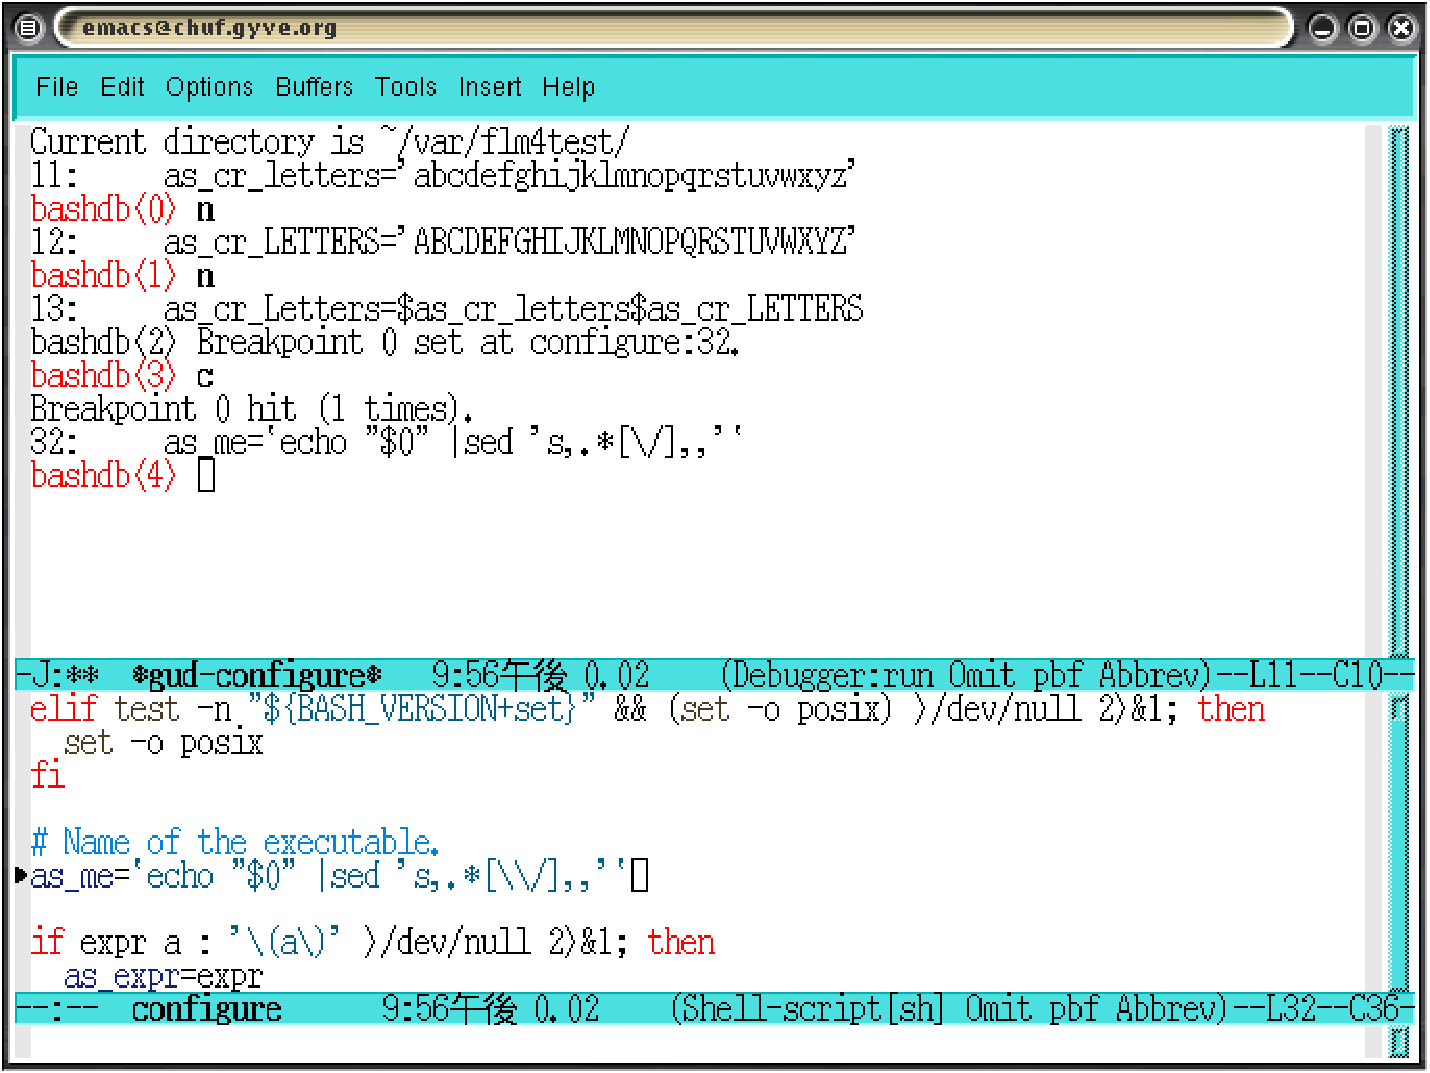
\includegraphics[width=\textwidth]{./images/bashdb-break_invert}
	\caption{Bash Debugger -- Break point \cite{bashdb}}
	\label{fig:bashdb}
\end{figure}

Bash Debugger má výhodu v~tom, že sám je napsaný v~Bashi. Je tak velice snadné zasahovat do běžícího skriptu svými příkazy.

Funkčnost debuggeru závisí na nastavení \texttt{DEBUG trap}, která je spuštěna před každým příkazem. V~\texttt{DEBUG trap} se pokaždé zkontroluje, zdali nemá být skript pozastaven, nebo zda není registrovaná nějaká událost. Také \texttt{EXIT} a \texttt{INT trap} jsou nastavené, aby debugger běžel i po skončení, respektive po přerušení skriptu.



% todo: popsat jak funguje, co vsechno umi, nejake priklady
% \url{http://bashdb.sourceforge.net/}


\subsection{BashEclipse}

BashEclipse \cite{basheclipse} je plugin do integrovaného vývojového prostředí Eclipse. Pro svůj běh vyžaduje nainstalovaný editor ShellEd \cite{shelled}.

BashEclipse funguje také na \texttt{DEBUG trap}. Na začátek každého skriptu, který chceme debuggovat, musíme přidat speciální soubor \texttt{\_DEBUG.sh}. V~tomto souboru se nastaví spojení s~TCP/IP socketem ze souboru pro zařízení tcp localhost s~portem 3333, ze kterého se čtou příkazy, které se v~\texttt{DEBUG trap} vykonají.

Zbytek debuggeru je napsán jako doplněk Eclipse.

Ukázkou grafického prostředí z~Eclipse při debuggování shell skriptu přes BashEclipse je obrázek \ref{fig:bash_eclipse}.

\begin{figure}
	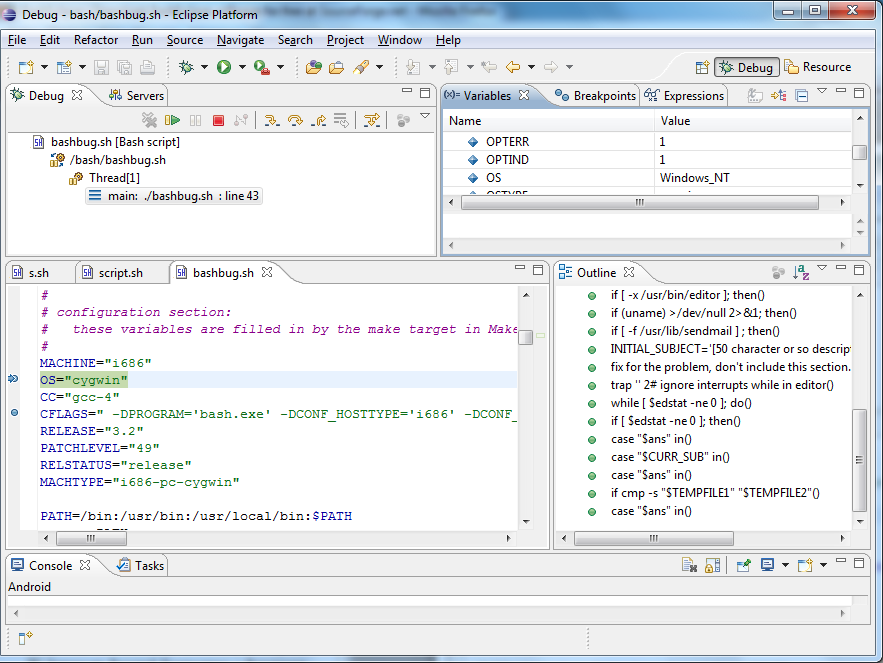
\includegraphics[width=1.0\textwidth]{./images/bash_eclipse}
	\caption{BashEclipse \cite{basheclipse}}
	\label{fig:bash_eclipse}
\end{figure}

% http://www.tldp.org/LDP/abs/html/devref1.html
% http://www.linuxjournal.com/content/more-using-bashs-built-devtcp-file-tcpip
% \url{http://unix.stackexchange.com/questions/131491/is-there-a-gui-debugger-for-shell-scripts}
% \url{https://sourceforge.net/projects/shelled/}
% \url{https://sourceforge.net/projects/basheclipse/}




%
%
%
%
%
\section{Možnosti debuggování v~interaktivním shellu}

Nebyl nalezen žádný externí nástroj pro debuggování interaktivního shellu. Nejčastějším postupem je však spouštění příkazů postupně. Pokud chce uživatel hledat chybu v~jednom příkazu, co spouští, může mu pomoci nastavení \texttt{xtrace}, aby například viděl, do jakých hodnot expandují proměnné.



%
%
\subsection{Definice debuggování v~interaktivním shellu}

%todo: nema cenu debugovat jednoduche prikazy, ale slozite ano. chceme umet rozkrokovat pipy a subshelly (tedy to co nam to dela ted)

Pro debuggování skriptů a programů existuje mnoho nástrojů, které definují, jaké operace a možnosti od takového nástroje očekáváme. Mezi takové základní operace patří možnost zastavit vykonávání skriptu nebo programu na určitém místě nebo za určitých podmínek. Po takovém zastavení by uživatel měl mít možnost zobrazit si další informace.

V~interaktivním shellu se zpravidla nespouštějí jednotlivé příkazy v~takovém množství, že by se mezi nimi chtěl uživatel zastavit. V~shellu lze příkazy spouštět v~rouře a v~takovém případě je vhodné vykonávání příkazu pozastavit a nechat si například vypsat výstup, který je následně určen jako vstup do dalšího programu.

I~v~interaktivním shellu se často setkáme s~použitím cyklů for a while. U~for cyklu uživatele může zajímat, přes jaké hodnoty iterátoru bude tělo cyklu spuštěno, popřípadě spustit tělo cyklu s~vlastním iterátorem.




\subsection{Možnosti realizování debuggeru interaktivního shellu}

Následující kapitoly shrnují možnosti, kterými by šel debugger interaktivního shellu implementovat.

Základní funkcionalita, která je nutná pro vytvoření takového programu, je ta, že příkazy napsané do shellu je možné nevykonat a místo toho spustit nějaký vlastní kód.

\subsection{GNU Readline}

GNU Readline umožňuje přemapovat klávesu enter tak, že se před i po řetězec znaků dopíšou nějaké další znaky. Myšlenka byla taková, že se příkaz obalí voláním funkce, ve které se příkaz spustí, popřípadě se zapne nějaký debugger nebo se vykonají jiné skripty.

Tuto myšlenku se podařilo implementovat, je vidět na ukázce \ref{lst:readline_hack}. V~této ukázce už je vidět modifikovaná řádka vstupu, ta se však objeví až po zmáčknutí klávesy enter. Příkaz bind říká, že po zmáčknutí klávesy enter se před vstup má vložit řetězec znaků \texttt{, '} a za vstup znak \texttt{'}. Znak \texttt{,} způsobí volání funkce s~názvem \texttt{,}, tento název byl zvolen tematicky jako název práce.

Bohužel má tento postup řadu nevýhod, z~nichž některé dělají celou myšlenku nepoužitelnou. Největší nevýhodou je, že nelze napsat víceřádkový příkaz, protože při psaní dalšího řádku zapůsobí obalovaní vstupu do funkce. Další nevýhodou je, že se příkaz ke spuštění změní, což může působit velice rušivě. Nevýhodou také je, že takto modifikovaný příkaz se uloží do historie, ale to je věc, která by šla ošetřit.

\noindent
\begin{minipage}{\linewidth}
\begin{lstlisting}[language=bash, caption={Modifikace Readline}, label={lst:readline_hack}]
bash-4.3$ ,() { echo "running: \"$@\""; eval "$@"; }
bash-4.3$ bind "RETURN: \"\e[1~, '\e[4~'\n\""
bash-4.3$ , 'echo test'
running: "echo test"
test
\end{lstlisting}
\end{minipage}

%
%
\subsection{Napsání nového REPLu}

Další možností, jak ovládat všechny příkazy k~vykonání, je napsat celý mechanismus, který se stará o~čtení příkazů, jejich vykonání a vypsání dalšího promptu. Takové smyčce se také říká REPL, z~anglického read-eval-print loop.

Základní implementace by mohla být velice jednoduchá a napsaná v~Bashi. Smyčka by mohla být součástí skriptu, který se pustí hned po startu Bashe.

Největší problém tohoto řešení je fakt, že uživatel není v~shellu, ale v~našem skriptu. To by mělo za následek například to, že by nastavené aliasy v~základu nefungovaly. Takových případů by se nashromáždilo víc a výsledkem práce by byla omezená verze shellu.

% https://brennan.io/2015/01/16/write-a-shell-in-c/
% https://www.gnu.org/software/libc/manual/html_node/Implementing-a-Shell.html#Implementing-a-Shell

%
%
\subsection{Patch do Bashe}

Celý mechanismus pro kontrolu příkazů a jejich nespouštění by mohl být napsán jako patch do zdrojového kódu Bashe. Přestože by takové řešení bylo nejrobustnější, instalace nového shellu je krok, který by mohl odradit nějaké uživatele.

%
\subsection{PS0}

\texttt{PS0} je prompt, který se zobrazí před  příkazem. Mechanismus pro kontrolu příkazů by mohl být spuštěn ze subshellu, který by byl vykonán při expanzi proměnné \texttt{PS0}. Problémem ale je, že ze subshellu není snadné interagovat s~hlavní instancí shellu.

%
%
\subsection{DEBUG trap}

DEBUG trap se spustí před vykonáním každého příkazu. Pokud je zapnutý pokročilý debuggovací mód pomocí extdebug a návratová hodnota DEBUG trap je nenulová, následující příkaz je přeskočen, tedy nevykonán.

Problém, který zde nastává, je ten, že DEBUG trap se spouští pro každý jednoduchý příkaz a ne pro celý vstup. Na ukázce \ref{lst:debugtrap} je nastavena DEBUG trap tak, že se vypíše zpracovávaný příkaz, který lze přeskočit.

\noindent
\begin{minipage}{\linewidth}
\begin{lstlisting}[language=bash, caption={DEBUG trap}, label={lst:debugtrap}]
bash-4.3$ trap 'echo "(trap: $BASH_COMMAND)"' DEBUG
bash-4.3$ echo foo | grep oo
(trap: echo foo)
(trap: grep oo)
foo
\end{lstlisting}
\end{minipage}

Pokud chceme spustit kód jen jednou pro celý vstup, můžeme použít trik, kdy nebudeme spouštět vůbec nic, tedy DEBUG trap vrátí vždy nenulovou hodnotu a v~první DEBUG trap spustit celý vstup pomocí příkazu eval. Tento vstup můžeme získat z~historie shellu, protože ta se uloží ještě před vykonáním příkazu.

Protože toto řešení bylo vybráno jako nejvhodnější, bylo realizováno. Detailní popis celého postupu je v~sekci \ref{sec:debugtraprealization}.


% https://bmizerany.github.io/roundup/


\section{Statická analýza skriptů}

Statická analýza skriptů znamená prozkoumat, analyzovat skript a například v~něm hledat nějaké problémy. Nejdůležitější je, že při této analýze není skript vykonáván.


%
%
\subsection{Vestavěná statická analýza}

Při volání skriptu Bashem můžeme použít parametr \texttt{-n} nebo použít příkaz \texttt{set -n}, kde \texttt{n} značí \texttt{noexec}, tedy mód, ve kterém se nebudou spouštět příkazy.

V~takovém módu lze nalézt syntaktické chyby, ale například se nekontroluje existence volaných příkazů. Tato metoda  tedy nepomůže proti překlepům.


%
%
\subsection{Check Bashisms}

Některé skripty chceme kvůli rychlosti spouštět v~Bourne-Shellu. Protože ten je pouze podmnožina Bashe, nástroj Check Bashisms \cite{checkbaskisms} najde výskyty takové syntaxe, která je podporovaná pouze v~Bashi a v~Bourne-Shellu nemusí fungovat správně.

Check Bashisms je skript napsaný v~jazyce Perl \cite{perl} a obsahuje sadu regulárních výrazů popisujících neportabilní syntaxi, které jsou hledané ve vstupním souboru.

% todo: ukazka?

% \url{https://sourceforge.net/projects/checkbaskisms/}
% https://linux.die.net/man/1/checkbashisms

%
%
\subsection{Explain Shell}

Projekt Explain Shell \cite{explainshell}, provádí statickou analýzu kódu, ale nehledá v~něm chyby, pouze vyparsuje vstupní kód a vyhledá příslušnou dokumentaci v~manuálových stránkách. Využívá se zde knihovny bashlex, která zde byla popsána v~sekci \ref{sec:bashlex}. Manuálové stránky, ze kterých se vybírá, jsou z~operačního systému Ubuntu.

% \url{http://www.explainshell.com/}

%
%
\subsection{ShellCheck}

ShellCheck \cite{shellcheck} je nástroj, který varuje před chybami a~dokonce dává návrhy na vylepšení ve skriptech v~Bashi, i~Bourne Shellu. Nástroj je dostupný jak online, tak jej lze snadno nainstalovat.

Shellcheck si dává za cíl tři základní věci. Za prvé pomoci nezkušeným uživatelům shellu, upozornit je na základní chyby srozumitelně, protože základní hlášení chyb v~shellu může působit zmateně.

Druhý cíl je vysvětlit nestandardní chování nebo neintuitivní syntaxi uživatelům kteří používající středně pokročilé praktiky.

Posledním cílem je upozornit pokročilé uživatele na okrajové případy a~nástrahy. Například skript může pracovat dobře, dokud nemá zpracovat soubor obsahující mezeru v~názvu.

ShellCheck obsahuje galerii špatného kódu s~přehledem základních chyb. Na jeho stránkách je však také podrobně popsán každý případ, který se hledá a na který se upozorňuje.

ShellCheck je napsaný v~čistě funkcionálním jazyce Haskell \cite{haskell} postaveném v~systému Cabal. Obsahuje parser, který tvoří abstraktní syntaktický strom. Zdroje chyb, varování a doporučení, které ShellCheck hledá, jsou kontrolovány jak při tvoření abstraktního syntaktického stromu, tak je zde i~soubor pravidel, ve kterých se hledá shoda s~příkazy na vstupu.

ShellCheck je velice aktivní projekt a~používá se často na testovacích serverech, jako je například Travis CI \cite{travisci}.
% TODO: cite cabal, travis ci

V~ukázce \ref{lst:shellcheck} je výpis ShellChecku pro ukázkový skript.

\noindent
\begin{minipage}{\linewidth}
\begin{lstlisting}[language=bash, caption={ShellCheck}, label={lst:shellcheck}]
bash-4.3$ ~/.cabal/bin/shellcheck ~/.commash/tmp/shellcheck_example.sh

In /home/n/.commash/tmp/shellcheck_example.sh line 5:
if (( $n > 3.5 )); then
      ^-- SC2004: $/${} is unnecessary on arithmetic variables.
           ^-- SC2079: (( )) doesn't support decimals. Use bc or awk.

In /home/n/.commash/tmp/shellcheck_example.sh line 9:
if [[ $1 == $n ]]; then
            ^-- SC2053: Quote the rhs of == in [[ ]] to prevent glob matching.
\end{lstlisting}
\end{minipage}

% https://www.linux.com/blog/shellcheck-code-check-shell-scripts
% http://www.dennyzhang.com/shellcheck/


%%%%%%%%%%%%%%%%%%%%%%%%%%%%%%%%%%%%%%%%%%%%%%%%%%%%%%%%%%%%%%%%%%%%%%%%%%%%%%%
\chapter{Realizace}

Cílem této práce má být multifunkční nástroj do interaktivní příkazové řádky. První funkcí je umět analyzovat příkazy před jejich vykonáváním, případně je nevykonat. Druhou funkcí je debugger, který umožní krokovat spouštěné příkazy nebo spouštět pouze jejich část. Poslední funkcí je sada příkazů, která obaluje základní příkazy z~GNU Coreutils a umožňuje vrátit změny provedené těmito příkazy, nebo rovnou uživateli vysvětlit, co přesně se stane a upozornit ho na jeho chyby.

Vytvořený nástroj se jmenuje Comma-shell a je to otevřený software. Nejaktuálnější zdrojové kódy, ukázky a návod na instalaci jsou na autorově veřejném Git repozitáři \cite{commash}.

%
\section{Virtuální stroj}

Pokud si chce uživatel vyzkoušet Comma-shell v~bezpečném a izolovaném prostředí, je dobrou praxí vytvořit si virtuální stroj pouze pro tento účel.

Instalace byla otestována na virtuálním stroji s~operačním systémem Debian verze \texttt{8.7.1-amd64}. Je nutné přidělit  minimálně 2GB operační paměti RAM, jinak je možné, že kompilace některých částí, zejména ShellChecku, skončí neúspěchem.

Virtuální stroj, který byl použit pro toto testování, je VirtualBox verze \texttt{5.0.32\_Ubuntu r112930}, pod operačním systémem založeným na Ubuntu 16.04 LTS.

% TODO na zacatku pisu o tom, ze zde bude postup instalace i nastaveni VM

% http://gensho.acc.umu.se/debian-cd/current/amd64/iso-cd/debian-8.7.1-amd64-lxde-CD-1.iso


\section{Instalace Comma-shellu}

Instalace Comma-shellu byla navrhnuta tak, aby byla co nejjednodušší. V~uká\-zce \ref{lst:csinstall} je příklad instalace v~operačním systému vycházejícího z~Debianu, například Ubuntu.

Nejprve se aktualizují a nainstalují potřebné balíčky. Proč jsou tyto konkrétní balíčky potřeba bude vysvětleno dále. Po nainstalování je dobré stáhnout aktuální verzi z~Githubu a spustit hlavní soubor. Ten zjistí, že Comma-shell není nainstalovaný a instalaci spustí.

\noindent
\begin{minipage}{\linewidth}
\begin{lstlisting}[language=bash, caption={Instalace Comma-shellu}, label={lst:csinstall}]
sudo apt update
sudo apt install git cabal-install python-pip xdotool -y
sudo pip install bashlex
git clone https://github.com/nesro/commash ~/.commash
source ~/.commash/comma.sh
\end{lstlisting}
\end{minipage}



%
%
%
%
%
% TODO sekce
\section{Nespouštění příkazů}\label{sec:debugtraprealization}
V~sekci realizování debuggeru interaktivního shellu bylo zmíněno několik možností. Pro realizaci bylo nakonec vybráno řešení s~\texttt{DEBUG trap}.

Celé řešení je postavené na tom, že \texttt{DEBUG trap} stále vrací nenulovou hodnotu, takže žádné příkazy nejsou vykonány.

Bash obsahuje proměnnou \texttt{PROMPT\_COMMAND}, která je vykonána před každým vypsání promptu. Comma-shell v~této proměnné volá funkci, která nastaví, že následující DEBUG trap je první v~pořadí po odeslání příkazu k~jeho vykonání.

\texttt{DEBUG trap}, která má vykonat nějaký kód, tak učiní pomocí funkce \texttt{eval}. \texttt{eval} je vestavěná funkce v~shellu, která vykoná příkaz, jenž ji byl předán argumentem.

\texttt{DEBUG trap} má informace pouze o~jednoduchém příkazu, který se má vykonat. Příkaz k~vykonání se uloží do historie ještě před zavoláním první \texttt{DEBUG trap}. Kód, který vykonává funkce \texttt{eval}, je tedy vzat jako ten poslední z~historie.

% TODO: implementovat minimalni verzi a ukazat ji tady?


%
%
%
%
%
\section{Hooks}

Hooks mají v~adresářové struktuře vyhrazenou vlastní složku, ze které se automaticky načtou všechny soubory. Comma-shell poskytuje funkce, s~nimiž lze zaregistrovat hook spouštěný před nebo po i s~jeho prioritou. Priorita slouží k~řazení posloupnosti hooků, protože bez nich by byly spouštěny v~pořadí abecedního seřazení podle názvů, což není vždy žádané.

Pokud hook spuštěný před příkazem vrátí nenulovou návratovou hodnotu, není následující příkaz vykonán. Vykonáváním příkazu v~tomto kontextu se nemyslí zabránění spuštění příkazu z~DEBUG trap, ale samotné vykonání příkazu přes eval v~první \texttt{DEBUG trap} po zobrazení promptu v~interaktivní příkazové řádce.

Díky této modularitě je velice jednoduché vytvořit vlastní kontroly příkazů ke spuštění. Je také možné vytvářet různé statistiky a logy akcí.


\subsection{Implementace hooků}

Při startu Comma-shell se vytvoří dvě pole. Jedno je určené pro hooky před a druhé pro hooky vykonávané po příkazu. Všechny soubory ze složky hooks vykonají pomocí příkazu source. V~hook souborech se pak volají příkazy, které přidají vstupní funkce hooků spolu s~jejich prioritou do předpřipravených polí.

Pokud se v~hlavní DEBUG trap má vykonat příkaz přes eval, jsou před ním zavolány všechny zaregistrované hooky. Pokud některý z~nich vrátí nenulovou hodnotu, příkaz se nevykoná. Pokud k~vykonání dojde, jsou následně zavolány všechny hooky určené po vykonání příkazu.

Vstupním funkcím hooku jsou předány dva argumenty. Prvním z~nich je časová známka, která je stejná pro všechny hooky a s~přesností na nanosekundy může sloužit jako jedinečný identifikátor příkazu. Druhým argumentem je jen spouštěný příkaz. Přestože si ho hook může sám přečíst z~historie, pokud bude vnitřní fungování v~budoucnu změněno, nebude problém se zpětnou kompatibilitou.

\subsection{Hooky před vykonáním příkazu}

Hooky před spuštěním příkazů mohou sloužit ke kontrole příkazu nebo například zaznamenání místa spuštění. Možné je jen vypsat nějaké doporučené používání příkazu, pokud je někde zvolen pracovní kodex.

\subsection{Hooky po vykonání příkazu}

Jednou z~nejdůležitějších věcí v~hooku spuštěném po příkazu je přístup k~návratovému kódu. Můžeme tak provádět akce závislé například na chybách příkazů.

\subsection{Předvytvořené hooky}

Comma-shell obsahuje v~základu několik předvytvořených hooků. Některé z~nich si zde popíšeme.


%
\subsection{ShellCheck hook}

ShellCheck na nástroj na kontrolu skriptů v~Bashi nebo Bourne Shellu. ShellCheck hook však vytvoří z~příkazu, který se má vykonat, skript, jenž následně ShellCheck zkontroluje. Pokud jsou nalezeny nějaké problémy, varování nebo doporučení, vypíše se uživateli zpráva, na základě které se může rozhodnout příkaz nespouštět, upravit nebo vypnout upozornění na danou chybu.

Protože ShellCheck je určen pro skripty, některé případy, na které upozorňuje, nejsou v~interaktivním shellu moc relevantní. ShellCheck například kontroluje, zda byl příkaz cd, který změní aktuální adresář, ošetřen tak, že pokud selže, skript se přizpůsobí. Například pokud se chce skript přepnout do nějaké složky a v~ní mazat soubory. Pokud příkaz cd selže v~interaktivním shellu, uživatel je o~situaci informován a může se podle toho zařídit.

\noindent
\begin{minipage}{\linewidth}
\begin{lstlisting}[language=bash, caption={ShellCheck}, label={lst:sccat}]
n@t:~$ cat x | grep y
,: ShellCheck:
cat x | grep y
    ^-- SC2002: Useless cat. Consider 'cmd < file | ..' or 'cmd file | ..' instead.
,: Now what? [r]un, [s]top, [i]gnore, [p]retype: s
,: Stopping the command.
\end{lstlisting}
\end{minipage}

\noindent
\begin{minipage}{\linewidth}
\begin{lstlisting}[language=bash, caption={ShellCheck}, label={lst:csfor}]
n@t:~$ for f in $(ls *.txt); do echo $f; done
,: ShellCheck:
for f in $(ls *.txt); do echo $f; done
         ^-- SC2045: Iterating over ls output is fragile. Use globs.
              ^-- SC2035: Use ./*glob* or -- *glob* so names with dashes won't become options.
                              ^-- SC2086: Double quote to prevent globbing and word splitting.
,: Now what? [r]un, [s]top, [i]gnore, [p]retype: s
,: Stopping the command.

\end{lstlisting}
\end{minipage}






% https://github.com/koalaman/shellcheck/wiki/SC2164

\subsection{Bashlex hook}

Bashlex hook je vstupní bod debuggeru. Pokud je debugger aktivní, tak se debugguje příkaz k~vykonání. Protože hooky před příkazem umí vykonávání příkazu přerušit, je právě hook vhodným místem pro volání debuggeru.

Celá část debuggeru bude popsána dále.

\subsection{Explain RC hook}

Explain RC hook je hook vykonávaný po skončení příkazu. Jedinou jeho funkcionalitou je, že pokud je návratová hodnota různá od nuly, vypíše hlášku o~nestandardní návratové hodnotě.

Ukázka \ref{lst:exprchook} ukazuje spuštění příkazu man s~neexistujícím příkazem. Přestože příkaz man sám o~sobě hlášku vypíše, hook vypíše další informace, které byly získány z~manuálové stránky příkazu man.

\noindent
\begin{minipage}{\linewidth}
\begin{lstlisting}[language=bash, caption={Explain RC hook}, label={lst:exprchook}]
n@t:~$ man noexistingcmd
No manual entry for noexistingcmd
,: return code warning: $? == 16 (At least one of the pages/files/keywords didn't exist or wasn't matched.)
\end{lstlisting}
\end{minipage}

Ukázka \ref{lst:exprchook2} zase ukazuje situaci, kdy byl příkaz ukončen klávesovou zkratkou Ctrl-C.

\noindent
\begin{minipage}{\linewidth}
\begin{lstlisting}[language=bash, caption={Explain RC hook}, label={lst:exprchook2}]
n@t:~$ cat
^C
,: return code warning: $? == 130 (Script terminated by Control-C)
\end{lstlisting}
\end{minipage}


\subsection{Notfound hook}

Když Bash hledá příkaz k~vykonání a nepodaří se mu ho najít, jako poslední možnost zkusí zavolat funkci command\_not\_found\_handle, které jako argument předá příkaz, který nebyl nalezen.

Comma-shell přepíše funkci command\_not\_found\_handle tak, aby nedělala nic, jen vrátila návratový kód 127. V~hooku spuštěném po příkazu se otestuje, zdali je návratová hodnota 127 a pokud ano, zavolá se kód obstarávající logiku, pokud příkaz není nalezen.

\noindent
\begin{minipage}{\linewidth}
\begin{lstlisting}[language=bash, caption={Explain RC hook}, label={lst:notfoundhook}]
n@t:~$ le asdf
,notfound: Command not found.
,notfound: [1] choose: "let asdf"
,notfound: [2] choose: "ln asdf"
,notfound: [3] choose: "ls asdf"
,notfound: [a]bort executing
,notfound: [e]dit the wrong command
,notfound: [p]re-type edited
,notfound: [s]uggest package for "le"
,notfound: [r]emove command from history
s
,notfound: executing: /usr/lib/command-not-found -- "le"
The program 'le' is currently not installed. You can install it by typing:
sudo apt install le
\end{lstlisting}
\end{minipage}

V~ukázce \ref{lst:notfoundhook} je vidět notfound hook v~akci. Uživatel může spustit příkaz, který zamýšlel, zastavit vykonávání, nechat si příkaz předepsat pro další úpravy,  nebo si nechat navrhnout instalaci balíčku odpovídající tomuto názvu.

%
%
%
%
%
\section{Implementace debuggeru v~interaktivním shellu}

V~následujících sekcích bude představen debugger určený do interaktivního shellu. Jedná se tedy o~takové použití, že uživatel chce krokovat, nebo částečně spouštět příkazy spouštěné v~interaktivním režimu shellu.

Implementace debuggeru je rozdělena na dvě části. První část je hook, který se spustí před příkazem a zjišťuje se v~něm, zdali má být debuggování aktivní. Pokud ano, je zavolán skript napsaný v~jazyce Python, ve kterém se použije knihovna Bashlex. Výstupem tohoto skriptu je na standardním výstupu informace pro uživatele, které možnosti má. Na chybovém výstupu jsou kódy v~shellu odpovídající jednotlivým akcím, které pak hook v~Comma-shellu vykoná po tom, co od uživatele přečte jeho požadovanou akci.

Použití knihovny Bashlex je velice jednoduché a intuitivní. Nejprve je celý vstup parsován a je vytvořen abstraktní syntaktický strom. Poté se projde celý strom znovu s~naší třídou, která definuje metody pro jednotlivé uzly. Příklad takové metody je \texttt{visitpipe}, která se zavolá, když se v~abstraktním syntaktickém stromě narazí na rouru. V~takové metodě máme přístup k~pozici roury a z~této informace můžeme uživateli nabídnout nějaké akce, třeba vykonat všechny příkazy až do té konkretní roury.


\section{Použití a možnosti debuggeru v~interaktivním shellu}

V~této kapitole budou ukázány některé možnosti použití debuggeru v~interaktivním shellu.

V~ukázce \ref{lst:dbginteractivesubhsell} je z~příkazové řádky spuštěn příkaz obsahující konstrukt subshellu. Tedy kód, který se vykoná v~nové instanci shellu. Demonstrativní příklad nejprve volá vestavěný příkaz \texttt{echo}, jehož argument, který je řetězec, obsahuje výstup ze subshellu s~voláním příkazu \texttt{date}, pro vypsání aktuálního roku. Pokud by uživatel chtěl zobrazit pouze obsah subshellu, musel by vykopírovat tu část příkazu jemu odpovídající a spustit. Debugger interaktivního shellu však dokáže tuto práci nejen urychlit, ale také ukáže, které součásti lze spustit samostatně.

\noindent
\begin{minipage}{\linewidth}
\begin{lstlisting}[language=bash, caption={Debugger interaktivního shellu -- subshell}, label={lst:dbginteractivesubhsell}]
n@t:~$ echo "the year is $(date +%Y)" | grep 2017
,: commash debugger:

echo "the year is $(date +%Y)" | grep 2017
                  ^-- [1] show substituion: $(date +%Y)
                               ^-- [2] show pipe flow: echo "the year is $(date +%Y)"

,: Select your option, [0] debug whole cmd, [q]uit, [r]un normally 1
,: Executing: "echo "$(date +%Y)""
2017

,: What now? [q]uit, [p]retype and debug just the next command
\end{lstlisting}
\end{minipage}

V~ukázce \ref{lst:dbginteractivepipe} je stejný příkaz jako v~ukázce \ref{lst:dbginteractivesubhsell}, ale uživatel provádí akci, kde si zobrazí výstup před druhou rourou.

\noindent
\begin{minipage}{\linewidth}
\begin{lstlisting}[language=bash, caption={Debugger interaktivního shellu -- subshell}, label={lst:dbginteractivepipe}]
n@t:~$ echo "the year is $(date +%Y)" | grep 2017
,: commash debugger:

echo "the year is $(date +%Y)" | grep 2017
                  ^-- [1] show substituion: $(date +%Y)
                               ^-- [2] show pipe flow: echo "the year is $(date +%Y)"

,: Select your option, [0] debug whole cmd, [q]uit, [r]un normally 2
,: Executing: "echo "the year is $(date +%Y)" "
the year is 2017

,: What now? [q]uit, [p]retype and debug just the next command
\end{lstlisting}
\end{minipage}

V~ukázce \ref{lst:dbginteractiveforcycle1} je příklad debuggování for cyklu. For cyklus se v~shellu často používá na provedení operace pro několik souborů, které jsou specifikované v~hlavičce for cyklu. Zde jsou tyto soubory označeny \texttt{*.txt}. Comma-shell debugger umožňuje zobrazit hodnoty, přes které bude postupně spuštěno tělo for cyklu.

\noindent
\begin{minipage}{\linewidth}
\begin{lstlisting}[language=bash, caption={Debugger interaktivního shellu -- výpis hodnot iterátoru for cyklu }, label={lst:dbginteractiveforcycle1}]
n@t:/tmp/csfor$ for i in *.txt; do echo "$i"; done
,: commash debugger:

for i in *.txt; do echo "$i"; done
    ^-- [1] show values of iterator: i
                   ^-- [2] run with custom iterator: echo "$i";

,: Select your option, [0] debug whole cmd, [q]uit, [r]un normally 1
,: Executing: "csit=0;for i in *.txt; do (( csit++ )); echo "( $csit ) i = $i"; done"
( 1 ) i = a.txt
( 2 ) i = b.txt
( 3 ) i = c.txt

,: What now? [q]uit, [p]retype and debug just the next command
\end{lstlisting}
\end{minipage}

V~další ukázce \ref{lst:dbginteractiveforcycle2} na ten samý for cyklus jako v~ukázce \ref{lst:dbginteractiveforcycle1} je tělo for cyklu spuštěno s~iterátorem, který interaktivně zapsal uživatel.

\noindent
\begin{minipage}{\linewidth}
\begin{lstlisting}[language=bash, caption={Debugger interaktivního shellu -- změna iterátoru for cyklu}, label={lst:dbginteractiveforcycle2}]
n@t:/tmp/csfor$ for i in *.txt; do echo "$i"; done
,: commash debugger:

for i in *.txt; do echo "$i"; done
    ^-- [1] show values of iterator: i
                   ^-- [2] run with custom iterator: echo "$i";

,: Select your option, [0] debug whole cmd, [q]uit, [r]un normally 2
,: Executing: "read -p "set iterator \"i\" value: " i; echo "$i";"
set iterator "i" value: test
test

,: What now? [q]uit, [p]retype and debug just the next command
\end{lstlisting}
\end{minipage}





\section{Implementace debuggeru shell skriptů}

Bash debugger je nejpoužívanější a zaběhlý debugger skriptů napsaných v~Bashi. Pracuje se s~ním stejně jako s~GNU GDB, takže práce s~ním může být snadná pro někoho, kdo s~GNU GDB má již zkušenosti. Bash debugger je založený na DEBUG trap, je tedy založený čistě na vnitřních nástrojích Bashe pro debuggování.

Comma-shell debugger shell skriptů se pro to snaží jít jinou cestou. Využívá podobných postupů, jako je Comma-shell debugger v~interaktivním shellu. Práce v~takovém debuggeru by měla být jednoduchá a natolik intuitivní, že není potřeba studovat žádnou manuálovou stránku. Příkazy, které je možné vykonat, budou zobrazeny v~menu a budou se spouštět zmáčknutím jedné klávesy.

Práce s~tímto debuggerem je taková, že je uživateli nabízeno menu pro každý příkaz první úrovně. Příkaz první úrovně je příkaz, který není v~žádné funkci, ani součástí smyček, nebo podmínek. V~takovém menu, pokud tomu příkaz odpovídá, je možné vstoupit do tohoto příkazu a v~něm krokovat příkazy.

V~ukázce \ref{lst:dbgscript} je příklad použití debuggeru na skript, který začíná for cyklem. Uživatel zvolí možnost krokovat cyklem s~vlastním iterátorem. Následně krokuje příkazy uvnitř tohoto for cyklu.

\noindent
\begin{minipage}{\linewidth}
\begin{lstlisting}[language=bash, caption={Debugger shell skriptu}, label={lst:dbgscript}]
n@t:~/.commash/script$ /home/n/.commash/script/commash_script.sh test.sh
,dbg: Next command:

for i in 1 2
do
	echo "another $i"
	uname
done

,dbg: Choose:
,dbg:    [1] show values of iterator: i
,dbg:    [2] run body with custom iterator: i
,dbg:    [3] step through iterations with custom iterator: i
,dbg:    [4] step in for body: i
,dbg:    [r]un
,dbg:    [q]quit
,dbg: eval begin
  ,dbg: stepping in for cycle
  ,dbg: set iterator "i" value: TEST
  ,dbg: Next command:

echo "another $i"

  ,dbg: Choose:
  ,dbg:    [r]un
  ,dbg:    [q]quit
  ,dbg: eval begin:

another TEST

  ,dbg: eval end
  ,dbg: Next command:

uname

  ,dbg: Choose:
  ,dbg:    [r]un
  ,dbg:    [q]quit
  ,dbg: eval begin:

Linux

  ,dbg: eval end
  ,dbg: input in context has ended
  ,dbg: stepping out for cycle

,dbg: eval end
\end{lstlisting}
\end{minipage}


Implementace je podobná jako v~Comma-shell debuggeru v~interaktivním shellu. Základem je parsovací knihovna Bashlex, která je spouštěna ve skriptu v~jazyce Python. Tento skript je volán ze skriptu v~Bashi, pro který jsou vráceny jak jednotlivé příkazy, tak i položky menu. S~každou položkou do menu je vrácen i kód, který je v~Bashi potom vykonán pomocí kostruktu eval.

Pokud se vstoupí do nějakého cyklu nebo podmínky, je hlavní část debuggeru zavolána rekurzivně na tělo podmínky nebo cyklu. Nastavování například iterátorů je zapsáno také jako kód v~Bashi, který se vykoná ještě před tímto rekurzivním voláním.


%
%
%
%
%
\section{Bezpečný mód}

Bezpečný mód umožňuje dvě základní věci. Tou jednodušší je pouze vypsání efektu příkazu, který má nějaké destruktivní následky. Druhá funkcionalita dovoluje vracení se do stavu před vykonáním příkazu.

Některé příkazy, jako například \texttt{rm} pro mazání souborů, mají zabudovanou nějakou ochranu před nechtěným spuštěním, ale ta je z~našeho pohledu buď nedostatečná, nebo je až moc striktní a zabírá příliš času, před samotným vykonáním příkazu.

Při navrhování bezpečných příkazů byl kladen důraz na myšlenku zobrazit uživateli nějaký souhrn akcí, co se stanou. Odsouhlasení základního chování by mělo být zmáčknutí pouze jedné klávesy. Při tom by mělo být možné nechat si vypsat nějaké detailnější informace, především pokud uživatel v~souhrnu uvidí něco, s~čím nepočítal, nebo co jej překvapilo.

Poslední důležitou věcí je nemít přepsané názvy nebezpečných příkazů na ty bezpečné z~Comma-shellu. V~takovém případě by si uživatel mohl zvyknout na dané chování a nebral by svoje akce jako absolutní. To by pro něj mohl být problém na systému, kde není Comma-shell s~bezpečnými příkazy nainstalován. Jak je vidět na ukázce \ref{lst:rmwrapp1}, v~základním nastavení se například název \texttt{rm} přepíše aliasem tak, aby informoval uživatele.

\noindent
\begin{minipage}{\linewidth}
\begin{lstlisting}[language=bash, caption={Přepsání nebezpečných příkazů}, label={lst:rmwrapp1}]
n@t:~$ rm test
,: Use ,rm for commash wrapper or /bin/rm for original rm.
\end{lstlisting}
\end{minipage}


%
\subsection{Comma-shell rm}

Příkaz \texttt{rm} z~balíčku GNU Coreutils obsahuje dva přepínače, které mají sloužit proti smazání nechtěných souborů. První přepínač \texttt{-i}, znamená výzvu před každým smazaným souborem. Jak je vidět na ukázce \ref{lst:rmwrapp2}, je potřeba skutečně odsouhlasit každý mazaný soubor.

\noindent
\begin{minipage}{\linewidth}
\begin{lstlisting}[language=bash, caption={rm}, label={lst:rmwrapp2}]
n@t:/tmp/rmtest$ mkdir -p dir
n@t:/tmp/rmtest$ touch {a..b}.txt dir/{c..d}.txt
n@t:/tmp/rmtest$ /bin/rm -ir ./*
/bin/rm: remove regular empty file './a.txt'? y
/bin/rm: remove regular empty file './b.txt'? y
/bin/rm: descend into directory './dir'? y
/bin/rm: remove regular empty file './dir/c.txt'? y
/bin/rm: remove regular empty file './dir/d.txt'? y
/bin/rm: remove directory './dir'? y
\end{lstlisting}
\end{minipage}

Druhý přepínač je \texttt{-I}. V~manuálových stránkách příkazu \texttt{rm} se píše, že je uživatel vyzván jednou, pokud odstraňuje tři nebo více souborů nebo pokud je mazána složka rekurzivně. U~tohoto přepínače je také napsáno, že je méně rušivý, než přepínač \texttt{-i}, ale stejně chrání před většinou chyb. V~ukázce \ref{lst:rmwrapp3} je vidět příklad použití tohoto přepínače. Přestože je uživatel upozorněn na to, že se bude něco mazat, už není upozorněn na to, co se bude mazat.

\noindent
\begin{minipage}{\linewidth}
\begin{lstlisting}[language=bash, caption={rm s~}, label={lst:rmwrapp3}]
n@t:/tmp/rmtest$ mkdir -p dir
n@t:/tmp/rmtest$ touch {a..b}.txt dir/{c..d}.txt
n@t:/tmp/rmtest$ /bin/rm -Ir ./*
/bin/rm: remove 3 arguments recursively? y
n@t:/tmp/rmtest$
\end{lstlisting}
\end{minipage}

Z~našeho pohledu jsou oba tyto přepínače v~praxi nepoužitelné. Jeden je moc striktní a druhý je zbytečný. Myšlenkou Comma-shell \texttt{rm} je zobrazit dostatečně komplexní souhrn toho, co se bude mazat, tak, aby se uživatel mohl rychle rozhodnout, zdali chce skutečně tyto soubory smazat, nebo se chce detailněji podívat na to, co všechno se bude mazat, například v~podsložkách.

Další funkcionalitou Comma-shell \texttt{rm} je schopnost obnovovat mazané soubory. Tato funkcionalita je zajištěna použitím koše ze specifikace Freedesktop \cite{freedesktop}. Pokud Comma-shell \texttt{rm} smaže nějaké soubory tak, že je přesune do koše, vytvoří soubor s~informací kdy, odkud a co bylo smazáno. Uživatel tedy má možnost nejen obnovit z~koše soubory, které potřebuje, ale je možné obnovit všechny soubory smazané jedním příkazem \texttt{rm}.

Implementace koše podle specifikace Freedesktop není úplně triviální, proto Comma-shell \texttt{rm} používá externí nástroj pro práci s~tímto košem, \texttt{trash--cli} \cite{trashcli}.

% https://github.com/andreafrancia/trash-cli
% https://www.freedesktop.org/wiki/Specifications/trash-spec/

V~ukázce \ref{lst:rmwrapp4} je příklad podobný \ref{lst:rmwrapp3} a \ref{lst:rmwrapp2}. Uživatel je informován o~tom, které soubory se budou mazat a po potvrzení trvalého smazání je spuštěn originální příkaz \texttt{rm}.

\noindent
\begin{minipage}{\linewidth}
\begin{lstlisting}[language=bash, caption={rm s~}, label={lst:rmwrapp4}]
n@t:/tmp/rmtest$ mkdir -p dir3
n@t:/tmp/rmtest$ touch {a..b}.txt dir3/{c..d}.txt f
n@t:/tmp/rmtest$ ,rm -r *
,rm: Files to remove:
,rm:    Directory: "dir3" (with 2 files)
,rm:    Removing file: "/tmp/rmtest/f"
,rm:    2 files with extension "txt"
,rm: Choose:
,rm:    [r]emove files
,rm:    [q]uit
,rm:    [t]rash files
,rm:    [s]how more files
r
,rm: /bin/rm -r a.txt b.txt dir3 f
\end{lstlisting}
\end{minipage}


V~ukázce \ref{lst:rmwrapp5} se maže složitější adresářová struktura a uživatel se rozhodl vypsat si více souborů ke smazání. Comma-shell \texttt{rm} vypisuje pouze obsah adresářů ze složky, ve které se začíná mazat, pro úplný seznam si už uživatel musí vypsat obsah adresáře sám.

\noindent
\begin{minipage}{\linewidth}
\begin{lstlisting}[language=bash, caption={rm s~}, label={lst:rmwrapp5}]
n@t:/tmp/rmtest$ mkdir -p dir3/dir4
n@t:/tmp/rmtest$ touch {a..b}.txt dir3/{c..d}.txt dir3/dir4/{e..f}.txt g
n@t:/tmp/rmtest$ ,rm -r *
,rm: Files to remove:
,rm:    Directory: "dir3" (with 3 files)
,rm:    Removing file: "/tmp/rmtest/g"
,rm:    2 files with extension "txt"
,rm: Choose:
,rm:    [r]emove files
,rm:    [q]uit
,rm:    [t]rash files
,rm:    [s]how more files
s
,rm: all files:
    a.txt
    b.txt
    dir3 (,: directory with 3 files)
        ./dir3/c.txt
        ./dir3/dir4 (,: directory with 2 files)
        ./dir3/d.txt
    g
,rm: Choose:
,rm:    [r]emove files
,rm:    [q]uit
,rm:    [t]rash files
,rm:    [s]how all files
q
\end{lstlisting}
\end{minipage}

V~ukázce \ref{lst:rmwrapp6} je použití Comma-shell \texttt{rm} pro přesunutí souborů do koše. Soubory se pomocí \texttt{trash--put} mažou postupně, včetně složek, aby bylo snadnější upozorňovat na chyby.

\noindent
\begin{minipage}{\linewidth}
\begin{lstlisting}[language=bash, caption={,rm -- přesouvání do koše}, label={lst:rmwrapp6}]
n@t:/tmp/rmtest$ mkdir -p dir3/dir4
n@t:/tmp/rmtest$ touch {a..b}.txt dir3/{c..d}.txt dir3/dir4/{e..f}.txt g
n@t:/tmp/rmtest$ ,rm -r *
,rm: Files to remove:
,rm:    Directory: "dir3" (with 3 files)
,rm:    Removing file: "/tmp/rmtest/g"
,rm:    2 files with extension "txt"
,rm: Choose:
,rm:    [r]emove files
,rm:    [q]uit
,rm:    [t]rash files
,rm:    [s]how all files
t
,rm trash: trying to trash: "/tmp/rmtest/a.txt" ok
,rm trash: trying to trash: "/tmp/rmtest/b.txt" ok
,rm trash: trying to trash: "/tmp/rmtest/dir3" ok
,rm trash: trying to trash: "/tmp/rmtest/g" ok
,rm trash: Done. Use ,t or ,trash handle trashed bundles
\end{lstlisting}
\end{minipage}

V~ukázce \ref{lst:rmwrapp7} je obnova souborů z~předchozí ukázky \ref{lst:rmwrapp6}. Po zavolání příkazu pro zobrazení balíčků smazaných souborů a vybrání jednoho podle času, místa a seznamu souborů si uživatel mimo jiné může nechat zobrazit detailní výpis souborů přesunutých do koše. Soubory může z~koše permanentně odstranit, nebo je obnovit. Pro odstranění se používá příkaz \texttt{trash--rm}. Pro obnovu souborů se používá příkaz \texttt{trash--restore}.

\noindent
\begin{minipage}{\linewidth}
\begin{lstlisting}[language=bash, caption={,rm -- obnova souborů }, label={lst:rmwrapp7}]
n@t:/tmp/rmtest$ ,t
,rm: This is a wrapper. Real trash is located at ~/.local/share/Trash
,rm: Choose the bundle:
    [1] ",rm -r *" from: /tmp/rmtest at 2017.04.28 20:06:38
    [q]uit
,rm: Chosen bundle 2017-04-28-20-06-38-461442374.
    [a]nother - select different bundle
    [s]how all trashed files
    [r]estore
    [d]iscard from the trash
    [q]uit
Showing all deleted files:
    -rw-rw-r-- 1 n n 0 dub 28 20:06 /tmp/rmtest/a.txt
    -rw-rw-r-- 1 n n 0 dub 28 20:06 /tmp/rmtest/b.txt
    drwxrwxr-x 3 n n 4096 dub 28 19:21 /tmp/rmtest/dir3
    -rw-rw-r-- 1 n n 0 dub 28 20:06 /tmp/rmtest/g
,rm: Chosen bundle 2017-04-28-20-06-38-461442374.
    [a]nother - select different bundle
    [s]how all trashed files
    [r]estore
    [d]iscard from the trash
    [q]uit
restore
,rm: restoring /tmp/rmtest/a.txt
,rm: restoring /tmp/rmtest/b.txt
,rm: restoring /tmp/rmtest/dir3
,rm: restoring /tmp/rmtest/g
,rm: bundle restored.
\end{lstlisting}
\end{minipage}


\subsection{Další bezpečné příkazy}

Cílem práce bylo implementovat základní příkazy ze sady GNU Coreutils, podobně jako právě Comma-shell \texttt{rm}. Tyto příkazy zde budou popsány pouze stručně a bez ukázek, protože jsou velice podobné Comma-shell \texttt{rm}.

Příkaz \texttt{chmod} slouží ke změně přístupových práv k~souboru. Před provedením příkazu \texttt{chmod} se uloží práva pomocí příkazu \texttt{getfacl} do souboru. Pro navrácení práv do původního stavu slouží opačný příkaz, \texttt{setfacl}, který umí práva obnovit z~toho souboru vytvořeného příkazem \texttt{getfacl}. Ukázka tohoto postupu je v~\ref{lst:sgfacl}

\noindent
\begin{minipage}{\linewidth}
\begin{lstlisting}[language=bash, caption={Kombinace příkazů \texttt{getfacl} a \texttt{setfacl}}, label={lst:sgfacl}]
n@t:/tmp/sgfacl$ touch a
n@t:/tmp/sgfacl$ getfacl a | tee log
# file: a
# owner: n
# group: n
user::rw-
group::rw-
other::r--

n@t:/tmp/sgfacl$ setfacl --restore=log
\end{lstlisting}
\end{minipage}

Příkaz \texttt{chown} umí měnit vlastníka souboru a skupinu, do které patří. Přestože by i zde mohl být pro obnovu použit příkaz \texttt{getfacl}, který také ukládá vlastníka a skupinu, příkaz \texttt{setfacl} už tyto vlastnosti nastavit neumí. Byl proto zvolen příkaz \texttt{find}, jehož výstup byl nastaven tak, aby jej bylo snadné číst ve smyčce, která bude tyto vlastnosti znovu nastavovat. 

% chgrp, chmod a chown

Příkazy jako \texttt{cp} a \texttt{mv} neukládají další extra informace, kromě spuštěného příkazu, složky ze které byl příkaz spuštěn a seznamu souborů předaných argumenty. Pro navrácení do původního stavu se pro příkaz \texttt{cp} smaže původní cíl příkazu, kam se kopírovalo, pro navrácení příkazu \texttt{mv} se cíl přejmenuje, nebo přesune zpět na původní místo.

% Za druhé jsou to příkazy cp, ln, mv, mkdir

% http://lingrok.org/xref/coreutils/src/

%\section{Historie}
%Popsat jak jsem vyresil ukladani historie prikazu, ukladani vystupu, navratove kody, jak vracet nasledky prikazu do puvodniho stavu.
%todo: historie taky neni v zadani a moc jsem to nedoresil. teoreticky by na to sel napsat pre a post hook, ktery zaznamena vsechno potrebne a zapise to nekam do souboru.
%todo: slo by snadno udelat: podobna historie co je ted, jen se ulozi odkud se prikaz spustil


% ----------------------------------------------------------------------------
%
% TESTOVANI
%
% ----------------------------------------------------------------------------
\chapter{Testování}

%
\section{Jednotkový test}

Jednotkový test, anglicky unit test, je metoda testování softwaru, při které jsou kontrolovány individuální jednotky zdrojového kódu na funkčnost.

%
\subsection{Testování shell skriptů}

Ukážeme si zde dva způsoby testování shell skriptů.

Tím prvním jsou klasické jednotkové testy, kdy se skripty testují přes jejich rozhraní, které nabízí. Jsou to buď jednotlivé funkce, nebo celé skripty.

Druhým způsobem je testování, které simuluje uživatele v~příkazové řádce a následně se testuje výstup pro určité řetězce. Tento postup je vhodný, pokud je hlavním cílem testování správná interakce v~příkazové řádce a nikoli jen spouštění skriptu. Příkladem takového testování může být připojení se na vzdálený počítač a spuštění nějakých příkazů.


% https://www.ibm.com/developerworks/community/blogs/brian/entry/when_to_use_expect_scripting_and_when_to_avoid_it10?lang=en

\section{shUnit2}

Projekt shUnit2 \cite{shunit2} je framework pro tvorbu unit testů, z~rodiny frameworků xUnit \cite{xunit}. Framework nabízí funkce na testování podmínek, jako například test, zdali se dvě hodnoty rovnají. Tyto funkce potom uživatel může použít ve svých funkcích pro zjištění, jestli jeho kód funguje správně.

Framework spouští funkce, které napsal uživatel, vyhledává funkce pro jednorázové nastavení a závěrečné čistění, ale také nastavení a čištění před každou uživatelskou funkcí.

% https://github.com/kward/shunit2

%\section{roundup}
% https://github.com/bmizerany/roundup

\section{Bats -- Bash Automated Testing System}
Bats \cite{bats} je framework pro Bash, který splňuje specifikaci TAP, Test Anything Protocol \cite{tap}. Jedná se o~protokol, který sjednocuje výsledky testů různých jazyků a tím usnadňuje jejich automatizaci.

Příklad testu Bats je v~ukázce \ref{lst:bats}. Jednotlivé testy jsou v~test blocích uvozených příkazem @test a popiskem testu. V~takovém bloku lze volat externí skripty nebo funkce příkazem run. Bats při tom naplní obsah proměnných tak, že obsahují návratové kódy, výstup jako celek, nebo pole jednotlivých řádek, pomocí kterých může uživatel kontrolovat, zdali byl jeho skript nebo funkce úspěšná.

\noindent
\begin{minipage}{\linewidth}
\begin{lstlisting}[language=bash, caption={Bats}, label={lst:bats}]
@test "A test which should run" {
  if [ foo != bar ]; then
    skip "foo isn't bar"
  fi

  run foo
  [ "$status" -eq 0 ]
}
\end{lstlisting}
\end{minipage}

% http://testanything.org/



%
\section{Automatizované spouštění příkazů}

Někdy chceme testovat chování, které se obtížně testuje unit testy. Existují pro to nástroje, které simulují chování reálného uživatele.

% Popsat jak se dají automaticky spouštět příkazy. Ať už lokálně, nebo vzdáleně. Popsat jak rekonstrukci z typescriptu, tak treba Tcl, Expect.

\subsection{Expect}

Expect \cite{expect} je rozšířením jazyka Tcl \cite{tcl}. Hlavním účelem je automatizace interakcí s~programy, které nabízejí nějakou formu textového terminálového uživatelského rozhraní.

Expect byl napsán Donem Libesem pro operační systémy z~rodiny Unix, ale později se dostal i na systémy Microsoft Windows a další.

Základní práce v~jazyce Expect je spouštění programů, například Bash nebo SSH. Do takovýchto instancí je možné posílat vstup stejně tak, jako by ho uživatel psal na klávesnici. Expect potom obsahuje konstrukce pro očekávání nějakého výstupu, podle kterého se může větvit zbytek skriptu.

% https://www.nist.gov/services-resources/software/expect
% http://expect.sourceforge.net/
% ISBN 1-56592-090-2
% http://shop.oreilly.com/product/9781565920903.do
% https://thepiratebay.org/torrent/7679076/Exploring_Expect_V413HAV


\subsection{Testování Comma-shellu}

Pro testování byl zvolen skriptovací jazyk Expect. Lze tedy velice snadno otestovat chování Comma-shellu a jeho částí pro různé vstupy.

Testy se skládají ze vstupů a z~řetězců, které se očekávají na výstupu. Přes Expect se potom vytvoří nová instance Bashe, ve které se automaticky načte Comma-shell a postupně se posílají vstupy a sledují se výstupy pro očekávané řetězce.

Testy jsou rozdělené na menší části, kde každá testuje jednu konkrétní věc. Přes skript lze pustit sérii všech testů.

V~ukázce \ref{lst:expectshellcheck} je část testu v~Expectu, která testuje, zdali se pro příkaz zavolá ShellCheck a příkaz se po zmáčknutí klávesy \texttt{r} skutečně spustí.

% todo: lepsi priklad?

\noindent
\begin{minipage}{\linewidth}
\begin{lstlisting}[language=tcl, caption={Expect test}, label={lst:expectshellcheck}]
spawn bash

send "var=content\n"
send "echo itis\$var\n"

expect {
	timeout {
		puts "CS_EXPECT_TIMEOUT 1 test_shellcheck.tcl"
		exp_continue
	}
	",: ShellCheck:" {
		puts "\nPASS 1"
	}
}

send "r"

expect {
	timeout {
		puts "CS_EXPECT_TIMEOUT 2 test_shellcheck.tcl"
		exp_continue
	}
	"itiscontent" {
		puts "\nPASS 2"
		exit 0
	}
}
\end{lstlisting}
\end{minipage}



%\subsection{Testování Hooks}

%\subsection{Testování Bezpečných příkazů}

%\subsection{Měření paměťových nároků}

% ----------------------------------------------------------------------------
%
% ZAVER
%
% ----------------------------------------------------------------------------
\begin{conclusion}

Byl vytvořen nástroj Comma-shell, který zlepšuje práci v~interaktivním shellu nejen novým uživatelům. Nabízí prostředí pro psaní uživatelských skriptů, hooků, před a po vykonání příkazu. Jeden předpřipravený hook, ShellCheck, umí kontrolovat příkazy před jejich vykonáváním a tím varovat uživatele před chybami. Dalším užitečným nástrojem je debugger příkazů spouštěných z~příkazové řádky. Lze je spouštět po částech, které dávají smysl a pomáhá tak zefektivnit práci při hledání chyb. Poslední částí je sada příkazů vylepšujících základní příkazy z~GNU Coreutils. Tyto příkazy jsou více přívětivější k~uživateli zobrazováním více informací a umí vrátit zpět provedené změny.

Comma-shell je frameworkem, který dává nové možnosti pro implementaci užitečných nástrojů do interaktivního shellu. Existují nástroje pro zobrazování informací v~shellu, ale chyběl zde nástroj pro komplexní analýzu příkazu ještě před jeho vykonáním a tím je právě Comma-shell.


\section{Možnost využití}

Comma-shell využije nejen začátečník, ale i zkušený uživatel. Přestože to v~takto rané fázi projektu zřejmě nebude, v~budoucnu by například bylo možné, aby se ve firmách nebo školících zařízeních připravil Comma-shell tak, aby zajistil bezpečnost a informoval uživatele.


\section{Další práce}

Účelem frameworku Comma-shell bylo připravit prostředí pro další vývoj. Toto prostředí funguje dobře a až na opravu případných chyb jej není potřeba příliš rozšiřovat. Je možné, že se v~budoucích verzích Bashe objeví nové debuggovací nástroje, takže bude možné jádro Comma-shellu přepsat.

Comma-shell debugger a sada bezpečných příkazů mají přirozeně místo pro další vývoj a vylepšování. Především to bude reagování na podněty uživatelů. Dále to může být přidávání funkcionality pro více přepínačů, nebo přidání podpory pro další příkazy z~GNU Coreutils.


\end{conclusion}

% ----------------------------------------------------------------------------


\bibliographystyle{csn690}
\bibliography{mybibliographyfile}

\appendix

\chapter{Seznam použitých zkratek}
% \printglossaries
\begin{description}
	\item[sh] Bourne Shell
	\item[bash] Bourne Again Shell
	\item[dash] Debian Almquist Shell
	\item[csh] C Shell
	\item[ksh] Korn Shell
	\item[zsh] Z~Shell
	\item[gnu] GNU's Not Unix
	\item[repl] Read–eval–print loop
	\item[cmd] Command
\end{description}


% % % % % % % % % % % % % % % % % % % % % % % % % % % %
% % Tuto kapitolu z výsledné práce ODSTRAŇTE.
% % % % % % % % % % % % % % % % % % % % % % % % % % % %
%
% \chapter{Návod k~použití této šablony}
%
% Tento dokument slouží jako základ pro napsání závěrečné práce na Fakultě informačních technologií ČVUT v~Praze.
%
% \section{Výběr základu}
%
% Vyberte si šablonu podle druhu práce (bakalářská, diplomová), jazyka (čeština, angličtina) a kódování (ASCII, \mbox{UTF-8}, \mbox{ISO-8859-2} neboli latin2 a nebo \mbox{Windows-1250}).
%
% V~české variantě naleznete šablony v~souborech pojmenovaných ve formátu práce\_kódování.tex. Typ může být:
% \begin{description}
% 	\item[BP] bakalářská práce,
% 	\item[DP] diplomová (magisterská) práce.
% \end{description}
% Kódování, ve kterém chcete psát, může být:
% \begin{description}
% 	\item[UTF-8] kódování Unicode,
% 	\item[ISO-8859-2] latin2,
% 	\item[Windows-1250] znaková sada 1250 Windows.
% \end{description}
% V~případě nejistoty ohledně kódování doporučujeme následující postup:
% \begin{enumerate}
% 	\item Otevřete šablony pro kódování UTF-8 v~editoru prostého textu, který chcete pro psaní práce použít -- pokud můžete texty s~diakritikou normálně přečíst, použijte tuto šablonu.
% 	\item V~opačném případě postupujte dále podle toho, jaký operační systém používáte:
% 	\begin{itemize}
% 		\item v~případě Windows použijte šablonu pro kódování \mbox{Windows-1250},
% 		\item jinak zkuste použít šablonu pro kódování \mbox{ISO-8859-2}.
% 	\end{itemize}
% \end{enumerate}
%
%
% V~anglické variantě jsou šablony pojmenované podle typu práce, možnosti jsou:
% \begin{description}
% 	\item[bachelors] bakalářská práce,
% 	\item[masters] diplomová (magisterská) práce.
% \end{description}
%
% \section{Použití šablony}
%
% Šablona je určena pro zpracování systémem \LaTeXe{}. Text je možné psát v~textovém editoru jako prostý text, lze však také využít specializovaný editor pro \LaTeX{}, např. Kile.
%
% Pro získání tisknutelného výstupu z~takto vytvořeného souboru použijte příkaz \verb|pdflatex|, kterému předáte cestu k~souboru jako parametr. Vhodný editor pro \LaTeX{} toto udělá za Vás. \verb|pdfcslatex| ani \verb|cslatex| \emph{nebudou} s~těmito šablonami fungovat.
%
% Více informací o~použití systému \LaTeX{} najdete např. v~\cite{wikilatex}.
%
% \subsection{Typografie}
%
% Při psaní dodržujte typografické konvence zvoleného jazyka. České \uv{uvozovky} zapisujte použitím příkazu \verb|\uv|, kterému v~parametru předáte text, jenž má být v~uvozovkách. Anglické otevírací uvozovky se v~\LaTeX{}u zadávají jako dva zpětné apostrofy, uzavírací uvozovky jako dva apostrofy. Často chybně uváděný symbol "{} (palce) nemá s~uvozovkami nic společného.
%
% Dále je třeba zabránit zalomení řádky mezi některými slovy, v~češtině např. za jednopísmennými předložkami a spojkami (vyjma \uv{a}). To docílíte vložením pružné nezalomitelné mezery -- znakem \texttt{\textasciitilde}. V~tomto případě to není třeba dělat ručně, lze použít program \verb|vlna|.
%
% Více o~typografii viz \cite{kobltypo}.
%
% \subsection{Obrázky}
%
% Pro umožnění vkládání obrázků je vhodné použít balíček \verb|graphicx|, samotné vložení se provede příkazem \verb|\includegraphics|. Takto je možné vkládat obrázky ve formátu PDF, PNG a JPEG jestliže používáte pdf\LaTeX{} nebo ve formátu EPS jestliže používáte \LaTeX{}. Doporučujeme preferovat vektorové obrázky před rastrovými (vyjma fotografií).
%
% \subsubsection{Získání vhodného formátu}
%
% Pro získání vektorových formátů PDF nebo EPS z~jiných lze použít některý z~vektorových grafických editorů. Pro převod rastrového obrázku na vektorový lze použít rasterizaci, kterou mnohé editory zvládají (např. Inkscape). Pro konverze lze použít též nástroje pro dávkové zpracování běžně dodávané s~\LaTeX{}em, např. \verb|epstopdf|.
%
% \subsubsection{Plovoucí prostředí}
%
% Příkazem \verb|\includegraphics| lze obrázky vkládat přímo, doporučujeme však použít plovoucí prostředí, konkrétně \verb|figure|. Například obrázek \ref{fig:float} byl vložen tímto způsobem. Vůbec přitom nevadí, když je obrázek umístěn jinde, než bylo původně zamýšleno -- je tomu tak hlavně kvůli dodržení typografických konvencí. Namísto vynucování konkrétní pozice obrázku doporučujeme používat odkazování z~textu (dvojice příkazů \verb|\label| a \verb|\ref|).
%
% \begin{figure}\centering
% 	
\includegraphics[width=0.5\textwidth, angle=30]{cvut-logo-bw}
% 	\caption[Příklad obrázku]{Ukázkový obrázek v~plovoucím prostředí}\label{fig:float}
% \end{figure}
%
% \subsubsection{Verze obrázků}
%
% % Gnuplot BW i barevně
% Může se hodit mít více verzí stejného obrázku, např. pro barevný či černobílý tisk a nebo pro prezentaci. S~pomocí některých nástrojů na generování grafiky je to snadné.
%
% Máte-li například graf vytvořený v programu Gnuplot, můžete jeho černobílou variantu (viz obr. \ref{fig:gnuplot-bw}) vytvořit parametrem \verb|monochrome dashed| příkazu \verb|set term|. Barevnou variantu (viz obr. \ref{fig:gnuplot-col}) vhodnou na prezentace lze vytvořit parametrem \verb|colour solid|.
%
% \begin{figure}\centering
% 	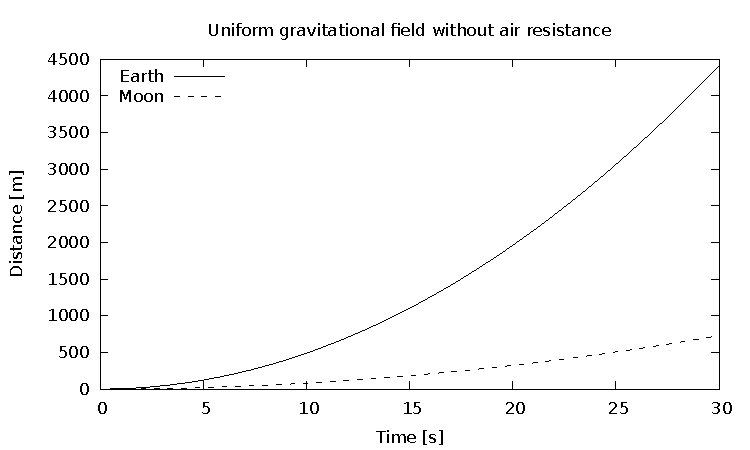
\includegraphics{gnuplot-bw}
% 	\caption{Černobílá varianta obrázku generovaného programem Gnuplot}\label{fig:gnuplot-bw}
% \end{figure}
%
% \begin{figure}\centering
% 	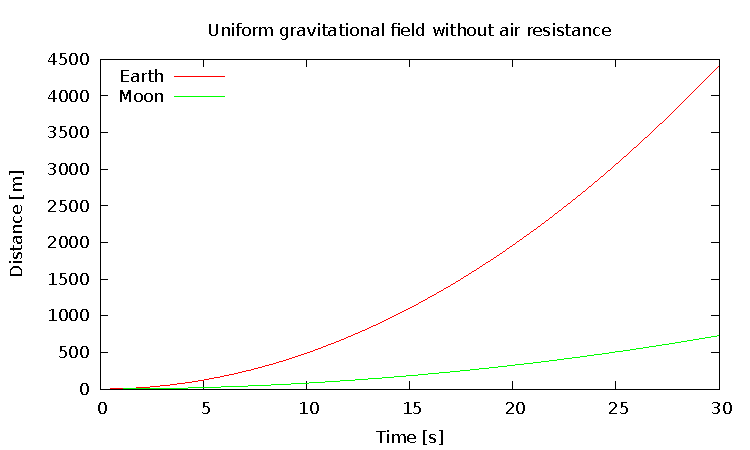
\includegraphics{gnuplot-col}
% 	\caption{Barevná varianta obrázku generovaného programem Gnuplot}\label{fig:gnuplot-col}
% \end{figure}
%
%
% \subsection{Tabulky}
%
% Tabulky lze zadávat různě, např. v~prostředí \verb|tabular|, avšak pro jejich vkládání platí to samé, co pro obrázky -- použijte plovoucí prostředí, v~tomto případě \verb|table|. Například tabulka \ref{tab:matematika} byla vložena tímto způsobem.
%
% \begin{table}\centering
% 	\caption[Příklad tabulky]{Zadávání matematiky}\label{tab:matematika}
% 	\begin{tabular}{|l|l|c|c|}\hline
% 		Typ		& Prostředí		& \LaTeX{}ovská zkratka	& \TeX{}ovská zkratka	\tabularnewline \hline \hline
% 		Text		& \verb|math|		& \verb|\(...\)|	& \verb|$...$|		\tabularnewline \hline
% 		Displayed	& \verb|displaymath|	& \verb|\[...\]|	& \verb|$$...$$|	\tabularnewline \hline
% 	\end{tabular}
% \end{table}
%
% % % % % % % % % % % % % % % % % % % % % % % % % % % %

\chapter{Obsah přiloženého CD}

%upravte podle skutecnosti

\begin{figure}
	\dirtree{%
		.1 readme.txt\DTcomment{stručný popis obsahu CD}.
		.1 commash\DTcomment{Git repozitář se zdrojovými kódy Comma-shellu}.
		.2 comma.sh\DTcomment{hlavní spouštěcí soubor}.
		.2 README.md\DTcomment{soubor s~instrukcemi pro instalaci}.
		.1 nesrotom-dip-2016\DTcomment{Git repozitář s~touto prací}.
		.2 DP\_Nesrovnal\_Tomas\_2016.pdf\DTcomment{text práce, formát PDF}.
		.2 DP\_Nesrovnal\_Tomas\_2016.tex\DTcomment{zdroj práce, formát \LaTeX{}}.
		.2 zadani\_DP\_Nesrovnal\_Tomas\_2016.pdf\DTcomment{zadání práce}.
	}
\end{figure}

\end{document}
